% Template file for an a0 landscape poster.
% Written by Graeme, 2001-03 based on Norman's original microlensing
% poster.
%
% See discussion and documentation at
% <http://www.astro.gla.ac.uk/users/norman/docs/posters/> 
%
% $Id: poster-template-landscape.tex,v 1.2 2002/12/03 11:25:46 norman Exp $


% Default mode is landscape, which is what we want, however dvips and
% a0poster do not quite do the right thing, so we end up with text in
% landscape style (wide and short) down a portrait page (narrow and
% long). Printing this onto the a0 printer chops the right hand edge.
% However, 'psnup' can save the day, reorienting the text so that the
% poster prints lengthways down an a0 portrait bounding box.
%
% 'psnup -w85cm -h119cm -f poster_from_dvips.ps poster_in_landscape.ps'

\documentclass[a0]{a0poster}
% You might find the 'draft' option to a0 poster useful if you have
% lots of graphics, because they can take some time to process and
% display. (\documentclass[a0,draft]{a0poster})

%%
%% MATH DEFINITIONS   
%%

\def\({\left(}
\def\){\right)}

\def\inv#1{{\frac{1}{#1}}}
\def\ddt#1{\der{#1}{t}}
\def\ddx#1{\der{#1}{x}}
\def\ddz#1{\der{#1}{z}}
\def\der#1#2{{\frac{d#1}{d#2}}}
\def\derder#1#2{{d^2\frac{#1}{d{#2}^2}}}
\def\norm#1{\labs #1 \rabs}
\def\pder#1#2{{\frac{\partial#1}{\partial#2}}}
\def\pderder#1#2{{\frac{\partial^2#1}{\partial{#2}^2}}}
\def\pdt#1{\pder{#1}{t}}
\def\pdx#1{\pder{#1}{x}}
\def\pdxx#1{\pderder{#1}{x}}
\def\pdz#1{\pder{#1}{z}}
\def\pdzz#1{\pderder{#1}{z}}
\def\ssize#1{{\scriptsize #1}}

\def\bmat{\left[ \begin{array}}
\def\bna{\begin{array}}
\def\bneas{\begin{eqnarray*}}
\def\bnea{\begin{eqnarray}}
\def\bnes{\begin{displaymath}}
\def\bne{\begin{equation}}

\def\emat{\end{array} \right]}
\def\ena{\end{array}}
\def\eneas{\end{eqnarray*}}
\def\enea{\end{eqnarray}}
\def\enes{\end{displaymath}}
\def\ene{\end{equation}} 

\def\half{\frac{1}{2}} 

\def\revrxn#1#2{
\begin{array}{c} 
{#1}\\
\rightleftharpoons \\
{#2}
\end{array}
}

\def\Bold#1{\vspace{0.1in} \noindent {\bf \boldmath #1}}

\def\Sec#1{Section~\ref{#1}}
\def\Secs#1#2{Sections~\ref{#1}--\ref{#2}}
\def\SecsAnd#1#2{Sections~\ref{#1} and \ref{#2}}

\def\Eqn#1{Eq.~\ref{#1}}
\def\Eqns#1#2{Eqs.~\ref{#1}--\ref{#2}}
\def\EqnsAnd#1#2{Eqs.~\ref{#1} and \ref{#2}}

\def\Eq#1{Eq.~\ref{#1}}
\def\Eqs#1#2{Eqs.~\ref{#1}--\ref{#2}}
\def\EqsAnd#1#2{Eqs.~\ref{#1} and \ref{#2}}

\def\Fig#1{Fig.~\ref{#1}}
\def\Figs#1#2{Figs.~\ref{#1}--\ref{#2}}
\def\FigsAnd#1#2{Figs.~\ref{#1} and \ref{#2}}

\def\Figure#1{Figure~\ref{#1}}
\def\Figures#1#2{Figures~\ref{#1}--\ref{#2}}
\def\FiguresAnd#1#2{Figures~\ref{#1} and \ref{#2}}

\def\avg#1{\langle{#1}\rangle}
\def\Parens#1{\left({#1}\right)}

\def\Bold#1{{\bf #1}}
\def\Block#1#2{{\bf #1:} {#2}\\ }

\def\bfcite#1{{\bf\cite{#1}}}

\def\bpi{\boldsymbol \pi}
\def\E{\mathsf E}
\def\P{\mathsf P}
\def\Pr{\mathsf P}
\def\Var{\mathsf{Var}}


%%%
%% CALCIUM DEFINITIONS   
%%

% My Definitions

\def\FcepsilonR1{Fc$\epsilon$R1}

\def\Ps{$\ps$}
\def\ps{{\rm s}^{-1}}

\def\Pms{$\pms$}
\def\pms{{\rm ms}^{-1}}

\def\UM{$\uM$}
\def\uM{\mu{\rm M}}

\def\Um{$\um$}
\def\um{\mu{\rm m}}

\def\Us{$\us$}
\def\us{\mu{\rm s}}

\def\Ums{$\ums$}
\def\ums{\mu{\rm m}^2}

\def\Nm{$\nm$}
\def\nm{\mu{\rm m}}

\def\Pumps{$\pumps$}
\def\pumps{\mu{\rm M}^{-1} {\rm s}^{-1}}

\def\Pumpms{$\pumpms$}
\def\pumpms{\mu{\rm M}^{-1} {\rm ms}^{-1}}

\def\UMps{$\uMps$}
\def\uMps{\mu{\rm M}/{\rm s}}

\def\Umpss{$\umpss$}
\def\umpss{\mu{\rm m}/{\rm s}^2}

\def\Umsps{$\umsps$}
\def\umsps{\mu{\rm m}^2/{\rm s}}

\def\Umspms{$\umspms$}
\def\umspms{\mu{\rm m}^2/{\rm ms}}

\def\Ryr{RyR}
\def\ip{{[{\rm IP}_3]}}

\def\Ip{${\rm IP}_3$}
\def\Ipr{${\rm IP}_3{\rm R}$}

\def\cad{[{\rm Ca}^{\rm 2+}]_{\rm d}}
\def\Cad{$\cad$}

\def\cabulk{[{\rm Ca}^{\rm 2+}]_{\rm bulk}}
\def\Cabulk{$\cabulk$}

\def\cainf{[{\rm Ca}^{\rm 2+}]_{\infty}}
\def\Cainf{$\cainf$}

\def\cai{[{\rm Ca}^{\rm 2+}]_{\rm i}}
\def\Cai{$\cai$}

\def\caext{[{\rm Ca}^{\rm 2+}]_{\rm ext}}
\def\Caext{$\caext$}

\def\cae{[{\rm Ca}^{\rm 2+}]_{\rm ER}}
\def\Cae{$\cae$}

\def\cat{[{\rm Ca}^{\rm 2+}]_{\rm T}}
\def\Cat{$\cat$}

\def\ve{{\varepsilon}}
\def\Bj{${\rm B}_j$}
\def\B{${\rm B}$}
\def\Bt{$\bt$}
\def\Ca{${\rm Ca}^{\rm 2+}$}
\def\K{${K}^{+}$}
\def\Cabj{${\rm CaB}_j$}
\def\Cab{${\rm CaB}$}
\def\Kj{$\kj$}
\def\Kjm{$\kjm$}
\def\Kjp{$\kjp$}
\def\Kmm{$\kmm$}
\def\Kkm{$\kkm$}
\def\Kmp{$\kmp$}
\def\Km{$\km$}
\def\Kp{$\kp$}
\def\bjt{\bj_T}
\def\b{[{\rm B}]}
\def\bj{[{\rm B}_j]}
\def\bmt{\bm_T}
\def\bt{\b_{\rm T}}
\def\bm{[B_m]}
\def\cabj{[{\rm CaB}_j]}
\def\cab{[{\rm CaB}]}
\def\ca{[{\rm Ca}^{2+}]}
\def\dc{D_c}
\def\dj{D_j}
\def\dm{D_m}
\def\db{D_b}
\def\kj{K_j}
\def\kjm{k^-_j}
\def\kjp{k^+_j}
\def\kmm{k^-_m}
\def\kmp{k^+_m}
\def\kkm{K_m}
\def\km{k^-}
\def\kp{k^+}

\def\wm{w^-}
\def\wp{w^+}
\def\minf{m_\infty}

% other ions

\def\mg{[{\rm Mg}^{2+}]}
\def\Mg{${\rm Mg}^{\rm 2+}$}





\pagestyle{empty}
\setcounter{secnumdepth}{0}

% The textpos package is necessary to position textblocks at arbitary 
% places on the page.
\usepackage[absolute]{textpos}

% Graphics to include graphics. Times is nice on posters, but you
% might want to switch it off and go for CMR fonts.
\usepackage{graphics,wrapfig,times}
\usepackage{color}


% These colours are tried and tested for titles and headers. Don't
% over use color!
\usepackage{color}
\definecolor{DarkBlue}{rgb}{0.1,0.1,0.5}
\definecolor{Red}{rgb}{0.9,0.0,0.1}

% Calcium defs
\def\Eq#1{Eq.~\ref{#1}}
\def\Eqs#1#2{Eqs.~\ref{#1}--\ref{#2}}
\def\EqsAnd#1#2{Eqs.~\ref{#1} and \ref{#2}}
\def\Figs#1{Figs.~\ref{#1}}
\def\bpi{\boldsymbol{\pi}} 
\def\E{\mathsf{E}} 
\def\Pr{\mathsf{P}} 
\def\Var{\mathsf{Var}} 
\def\Cov{\mathsf{Cov}} 
\def\be{\boldsymbol{e}} 
\def\beo{\boldsymbol{e}_\mathcal{O}}
\def\bec{\boldsymbol{e}_\mathcal{C}}
\def\io{I_\mathcal{O}}
\def\ic{I_\mathcal{C}}
\def\bu{\boldsymbol{u}} 
\def\bzero{\boldsymbol{0}} 
\def\bone{\boldsymbol{1}} 
\def\bx{\boldsymbol{x}} 
\def\by{\boldsymbol{y}} 
\def\bt{\boldsymbol{t}} 
\def\bk{\boldsymbol{k}} 
\def\bb{\boldsymbol{b}}
\def\diag{\mbox{diag}}
\def\c{\mathcal{C}}
\def\o{\mathcal{O}}
\def\r{\mathcal{R}}

\def\Ca{Ca$^{2+}$}

% see documentation for a0poster class for the size options here
\let\Textsize\normalsize
\def\Head#1{\noindent{\begin{center}\LARGE\color{DarkBlue} #1\end{center}}}
\def\LHead#1{\noindent{\LARGE\color{black} #1}\medskip}
\def\Subhead#1{\noindent{\large\color{black} #1}\medskip}
\def\Title#1{\noindent{\Huge\color{Red} #1}}

%\def\Head#1{\noindent\hbox to \hsize{\hfil{\LARGE\color{DarkBlue} #1}}\medskip}
%\def\Title#1{\noindent{\VeryHuge\color{Red} #1}}

% Set up the grid
%
% Note that [40mm,40mm] is the margin round the edge of the page --
% it is _not_ the grid size. That is always defined as 
% PAGE_WIDTH/HGRID and PAGE_HEIGHT/VGRID. In this case we use
% 23 x 12. This gives us three columns of width 7 boxes, with a gap of
% width 1 in between them. 12 vertical boxes is a good number to work
% with.
%
% Note however that texblocks can be positioned fractionally as well,
% so really any convenient grid size can be used.
%
\TPGrid[40mm,40mm]{23}{12}      % 3 cols of width 7, plus 2 gaps width 1

\parindent=0pt
\parskip=0.5\baselineskip

\usepackage{graphicx}
%\graphicspath{{figs/}}
\usepackage{amssymb}
\usepackage{amsmath, amsthm}

\begin{document}

% Understanding textblocks is the key to being able to do a poster in
% LaTeX. In
%
%    \begin{textblock}{wid}(x,y)
%    ...
%    \end{textblock}
%
% the first argument gives the block width in units of the grid
% cells specified above in \TPGrid; the second gives the (x,y)
% position on the grid, with the y axis pointing down.

% You will have to do a lot of previewing to get everything in the 
% right place.

% This gives good title positioning for a portrait poster.
% Watch out for hyphenation in titles - LaTeX will do it
% but it looks awful.
\begin{textblock}{23}(0,-0.36)
\centering
\Title{\Huge Modulation of local \Ca\ release and depletion signals through calsequestrin-mediated RyR luminal regulation}
%\Title{Measuring Chaos: Lyapunov and Box-Counting Dimensions}
\end{textblock}

\begin{textblock}{23}(0,0)
\centering
\LHead{Ryan Carpenter$^{1}$, S{\'a}ndor Gy{\"o}rke$^{2}$, Gregory D. Smith$^{1}$\\
}
\Subhead{
$^{1}$ Department\, of Applied Science, The College of William and Mary, Williamsburg, VA, 23187 \\
$^{2}$ Davis Heart \& Lung Research Institute, The Ohio State University, Columbus, OH, 43210\\
%$^{1}$ Dept.\,of Math.\,Sciences, U.\,S. Military Academy at West Point, West Point, NY, 10996 \\
%$^{2}$ Dept.\,of Applied Science \& $^{3}$ Dept.\,of Computer Science, College of William and Mary, Williamsburg, VA, 23187 \\
}
\end{textblock}

\begin{textblock}{1}(-0.35,-0.35)
\begin{figure}

\includegraphics[height=1in]{pics/WMlogo}
\end{figure}
\end{textblock}



\begin{textblock}{23}(21.9,-0.45)
\begin{figure}

\includegraphics[height=1.5in]{pics/Ohio_state_med}
\end{figure}
\end{textblock}

%\begin{textblock}{7}(0,1.52)
%
%\LHead{Funded by NSF CSUMS Grant: DMS 0703532}
%\end{textblock}



% Uni logo in the top right corner. A&A in the bottom left. Gives a
% good visual balance, but you may want to change this depending upon
% the graphics that are in your poster.


\begin{textblock}{5}(-0.25,0.30)
%\hrule\medskip
\Head{--- Abstract ---}
\vspace{-0.3in}


\begin{wrapfigure}{l}{6in}
\begin{center}

%\begin{picture}(280,340)(280,680)
%\put(180,660)
{\includegraphics*[height=5in]{pics/CSQ_binding}}
%\end{picture}
%\caption{\small {CAPTION}}
\label{fig:CSQ}
\end{center}
\end{wrapfigure}

Luminal regulation of ryanodine receptors (RyRs) is likely an important factor in \Ca\ release in cardiac myocytes. The \Ca-free form of cardiac calsequestrin (CSQ  or CASQ2 below), a luminal \Ca\ buffer, binds to the RyR/triadin/junctin complex and modulates spark activity. When jSR [\Ca] is low, CSQ binds to the channel and lowers the RyR open probability. We present hybrid Markov chain/ODE simulations of a release site consisting of 100 eight-state Lee-Keener RyRs and associated \Ca\ domain dynamics [1]. Below, we simulate different possible CSQ-RyR interactions. The resulting emergent spark properties are compared to experimental observations of spark activity in control cells and several arrhythmogenic CSQ mutants [2].


% This binding only occurs with the \Ca-free form of CSQ. 

%Luminal regulation of Ryanodine Receptors (RyRs) is an important factor in \Ca\ release in cardiac myocytes. Cardiac calsequestrin (CASQ2), a luminal \Ca\ buffer, binds to the RyR triadin junctin complex in order to modulate spark activity. However, CASQ2 binds to the RyR complex only when it is not bound to \Ca. Thus, when jSR [Ca] is low, CASQ2 binds to the channel and lowers the open probability of the channel. In an effort to model how CASQ2 affects the spontaneous activity of a cluster of RyRs, a Markov Chain representation of a release site compositionally defined of 100 Lee-Keener RyRs [1] involving interactions with CASQ2 was constructed simultaneously with a bidomain model of calcium release. The background nSR [\Ca] is fixed and determined by equilibrating the simulated time averaged release flux and calculated SERCA pump flux of our model. Different aspects of Calsequestrin are modeled and simulated in order to compare to experimental evidence of spark activity involving known arrhythmogenic CASQ2 mutants [2]. 

%Increases in the total amount of Calsequestrin lead to increased spark amplitudes as well as increased jSR recovery times. Interestingly, this also leads to increased blink nadirs. Varying the binding properties of CASQ2 to Ca leads to changes in spark amplitude and recovery times, as well as changes in background nSR [Ca]. Finally, changes in the binding properties of CASQ2 to the RyR is associated with changes in background nSR [Ca], but does not effect the recovery times of Ca blinks.
%Mathematical models of calcium release sites derived from Markov chain models of intracellular calcium channels exhibit collective gating reminiscent of the experimentally observed phenomenon of stochastic calcium excitability (i.e., calcium puffs and sparks).  We present a Kronecker structured representation using stochastic automata networks for calcium release site models and perform benchmark stationary distribution calculations using both exact and approximate iterative numerical solution techniques that leverage this structure.  We find multi-level methods provide excellent convergence with modest additional memory requirements.  When an exact solution is not feasible, iterative approximate methods based on the power method may be used, with performance similar to Monte Carlo estimates.  
\medskip
\end{textblock}

\begin{textblock}{1.5}(1,2.81)
\small Reproduced from [1]
\end{textblock}


\begin{textblock}{5}(-0.25,4.10)
%\hrule\medskip
\Head{--- Bidomain Model Description ---}

\begin{center}
\begin{figure}
\begin{picture}(280,340)(280,680)
\put(180,660){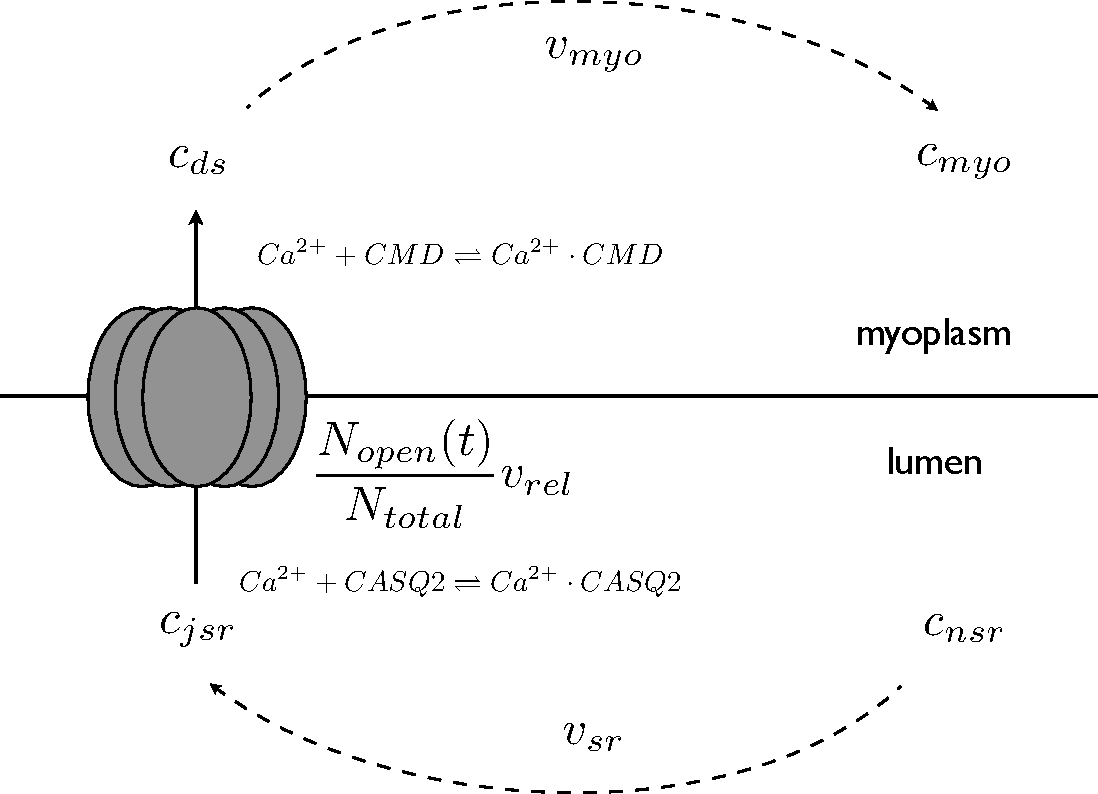
\includegraphics[height=5in]{pics/domains_poster_rotate}}
\end{picture}
%\caption{\small {Schematic representation of model components and fluxes. The model includes domain [\Ca] as well as bulk [\Ca]}}
\label{fig:domains}
\end{figure}
\end{center}

The evolution in time of the [\Ca] in the diadic subspace ($c_{ds}$) and jSR ($c_{jsr}$) is given by
\vspace{-0.2in}
$${\frac{dc_{ds}}{dt}} =\frac{\beta_{ds}}{\lambda_{ds}}(J_{ryr} - J_{efflux})  \qquad {\frac{dc_{jsr}}{dt}} =\frac{\beta_{jsr}}{\lambda_{jsr}}(J_{refill} - J_{ryr})$$ 
\vspace{-0.15in} where
%\vspace{-0.0in}
$$J_{efflux} =  {v_{myo}}(c_{ds} - c_{myo}) \qquad J_{refill} =  v_{sr}(c_{nsr} - c_{jsr})$$
$$J_{ryr} = \frac{N_{open}(t)}{N_{total}} (c_{jsr}- c_{ds}),$$
\vspace{-0.1in}
$\lambda_{ds}$ and $\lambda_{jsr}$ are volume fractions, and  $\beta_{jsr}$ and $\beta_{ds}$ are \Ca- dependent buffering factors. $N_{open}(t)$ is the number of open channels in the model \Ca\ release site composed of 100 stochastically gating Lee-Keener RyRs [1]. The channels are identical and coupled under the assumption that each experiences the same ds and jSR [\Ca]. We assume rapid equilibration of the free and bound forms of CSQ.
\vspace{-0.3in}
\begin{center}
\begin{figure}
\begin{picture}(200,450)(200,135)
\put(00,120){\includegraphics*[height=6in]{pics/8state_poster_new}}
%\put(-125,120){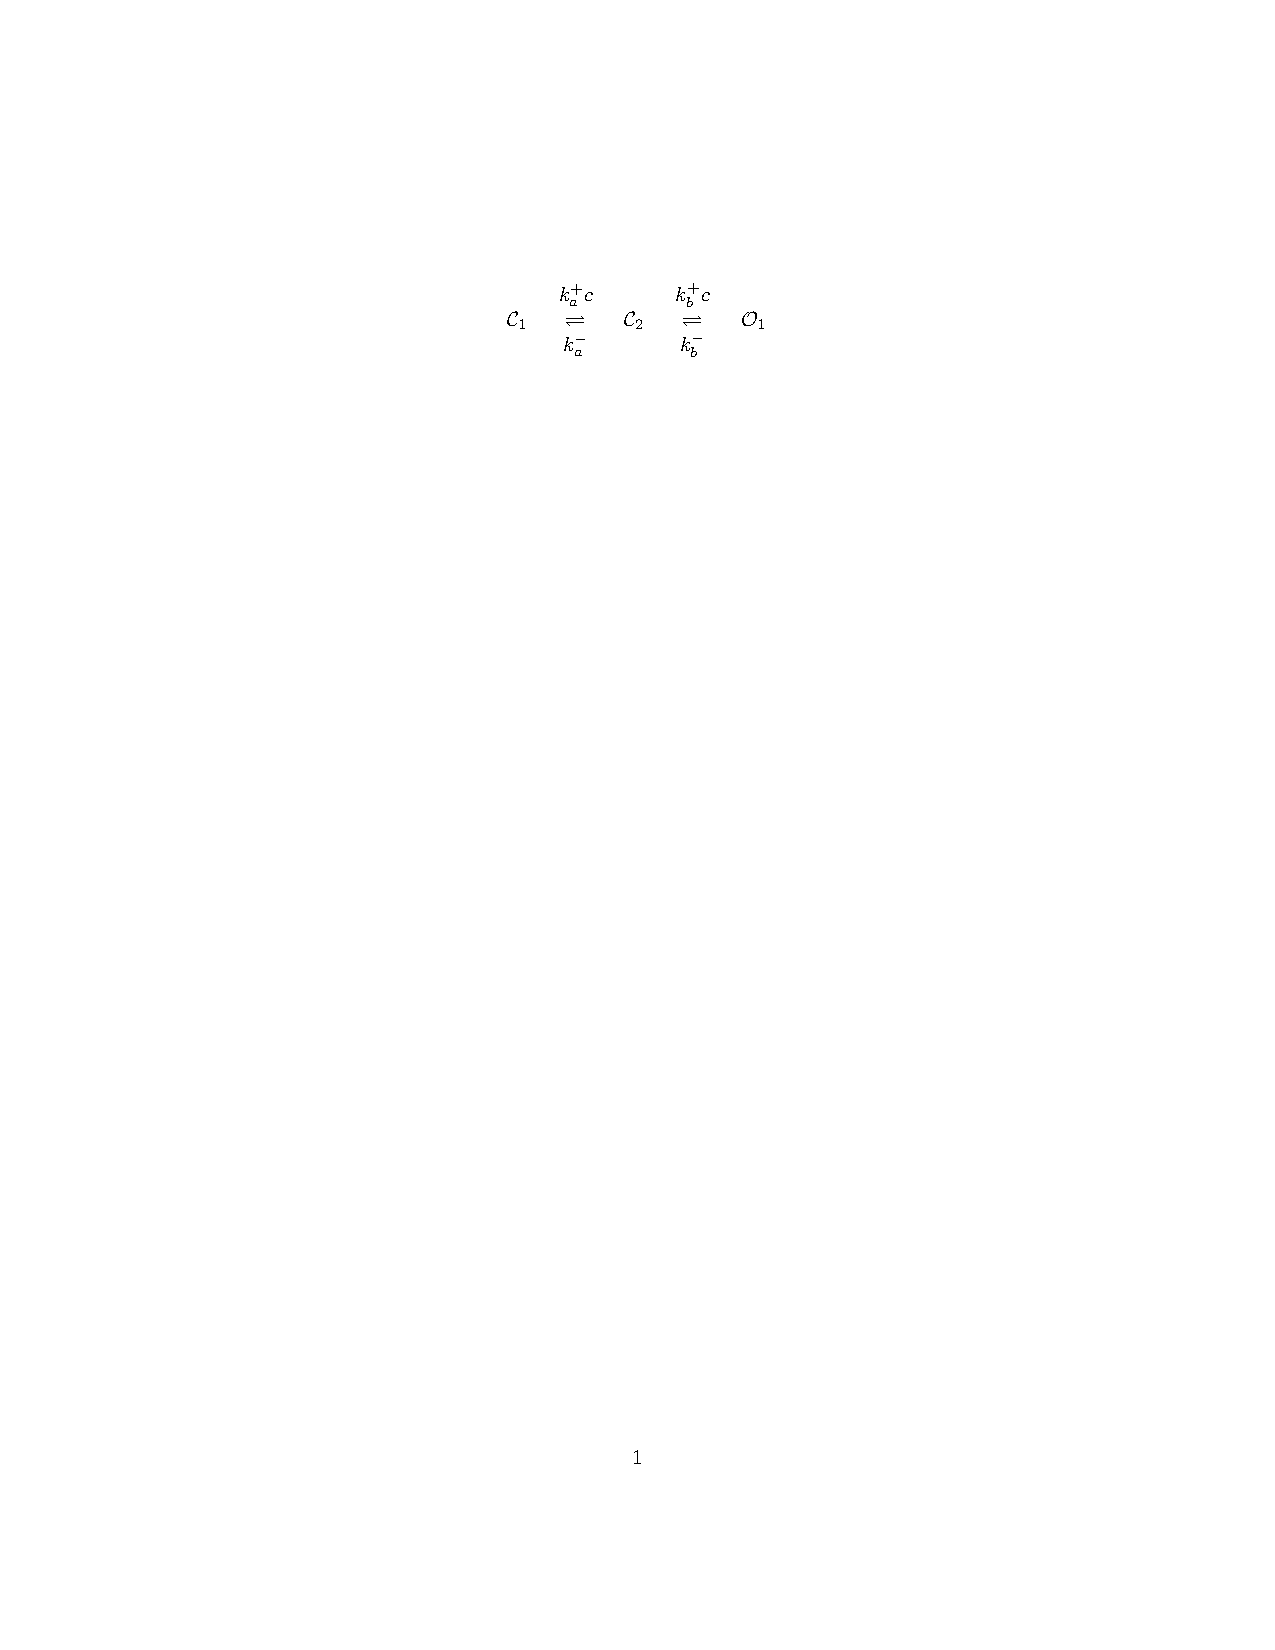
\includegraphics[height=1in]{pics/threestate}}

\end{picture}
\caption{The eight-state Lee-Keener RyR model [1]. $q$ represents the concentration of the \Ca-free form of CSQ.  We assume rapid equilibration between CSQ and the RyR.}
\label{fig:models}
\end{figure}
\end{center}

%\bigskip\hrule
\end{textblock}

%\begin{textblock}{7.5}(-0.25, 6.65)
%\hrule\medskip
%\Head{--- Model Setup: Exact Methods ---}
%\vspace{-0.1in}
%The generator matrix for a single 3- or 6-state channel model in Fig.~\ref{fig:sparks}(c)-(d) takes the form
%\[
%Q = K_- + \left( c_\infty I  + c_d \io \right) K_+ \label{QELEM}
%\]
%where $K_-$ and  $K_+ $ are $M \times M$ matrices that collect the unimolecular
%($k_i^-$) and bimolecular ($k_i^+$) transition rates, $M$ is the number of states in the single channel model, $I$ is the $M \times M$ identity matrix, $\io = \diag \left\{ \beo \right\}$, and $\beo$ is an $M \times 1$ vector indicating open states of the single channel model [2].  For example, for the 3-state model of \Fig{fig:sparks}(c) we have
%\vspace{-0.2in}
%\[
%K_- = \left(
%\begin{array}{ccc}
%0 & 0 & 0 \\
%k_a^- & -k_a^- & 0 \\
%0 & k_b^- & -k_b^- \\
%\end{array}
%\right),
%\quad\quad
%K_+ = \left(
%\begin{array}{ccc}
%- k_a^+ & k_a^+ & 0 \\
%0 & -k_b^+ & k_b^+ \\
%0 & 0 & 0 \\
%\end{array}
%\right).
%\]
%In the case of $N$ channels coupled at the \Ca\ release site, the
%expanded generator matrix---i.e., the SAN descriptor---is given by 
%\vspace{-0.2in}
%\begin{equation}
%\label{equ:kron}
%Q^{(N)} =  \bigoplus_{n=1}^N X_\infty + \sum_{i,j=1}^{N} \bigotimes_{n=1}^{N} X_{ij}^n
%\end{equation}
%where $X_\infty = K_-  + c_\infty K_+$ and
%\vspace{-0.2in}
%\[
%X_{ij}^n = \left\{ 
%\begin{array}{cl}
%\io & \mbox{for} \; i \neq j, \; i = n \\
%c_{ij} K_+ & \mbox{for} \; i \neq j, \; j = n \\
%c_{d}\io K_+ & \mbox{for} \; i = j = n \\
%I & \mbox{otherwise}. \\
%\end{array}
%\right.
%\]
%We are interested in calculating both the stationary distribution given by
%\[
%\bpi^{(N)} Q^{(N)} = \bzero \quad \mbox{subject to} \quad \bpi^{(N)} \be^{(N)} = 1
%\]
%and a coarser measure called the puff/spark {\it Score} defined as
%\begin{equation}
%\label{equ:score}
%Score = \frac{\mbox{Var}[f_\mathcal{O}]}{\mbox{E}[f_\mathcal{O}]}=\frac{1}{N}\frac{\mbox{Var}[N_\mathcal{O}]}{\mbox{E}[N_\mathcal{O}]}.
%\end{equation}

%\bigskip\hrule
%\end{textblock}

\begin{textblock}{6}(5.25, 0.8)
%\hrule\medskip
\Head{---Experimental results ---}


%\vspace{-.7in}
\begin{center}
\begin{figure}
\begin{picture}(280,340)(320,400)

%\put(140,260){\includegraphics*[height=7in]{pics/Poster_exper2}}
\put(50,200){\includegraphics*[height=7.5in]{pics/Poster_exper_cover}}



%\put(180,260){\includegraphics[height=5.5in]{pics/Experiment_color}}
%\put(180,260){\includegraphics[height=5.5in]{pics/Exper_snapshot}}
%\put(180,260){\includegraphics[height=5.5in]{pics/Exper_rotated}}
%\put(-125,120){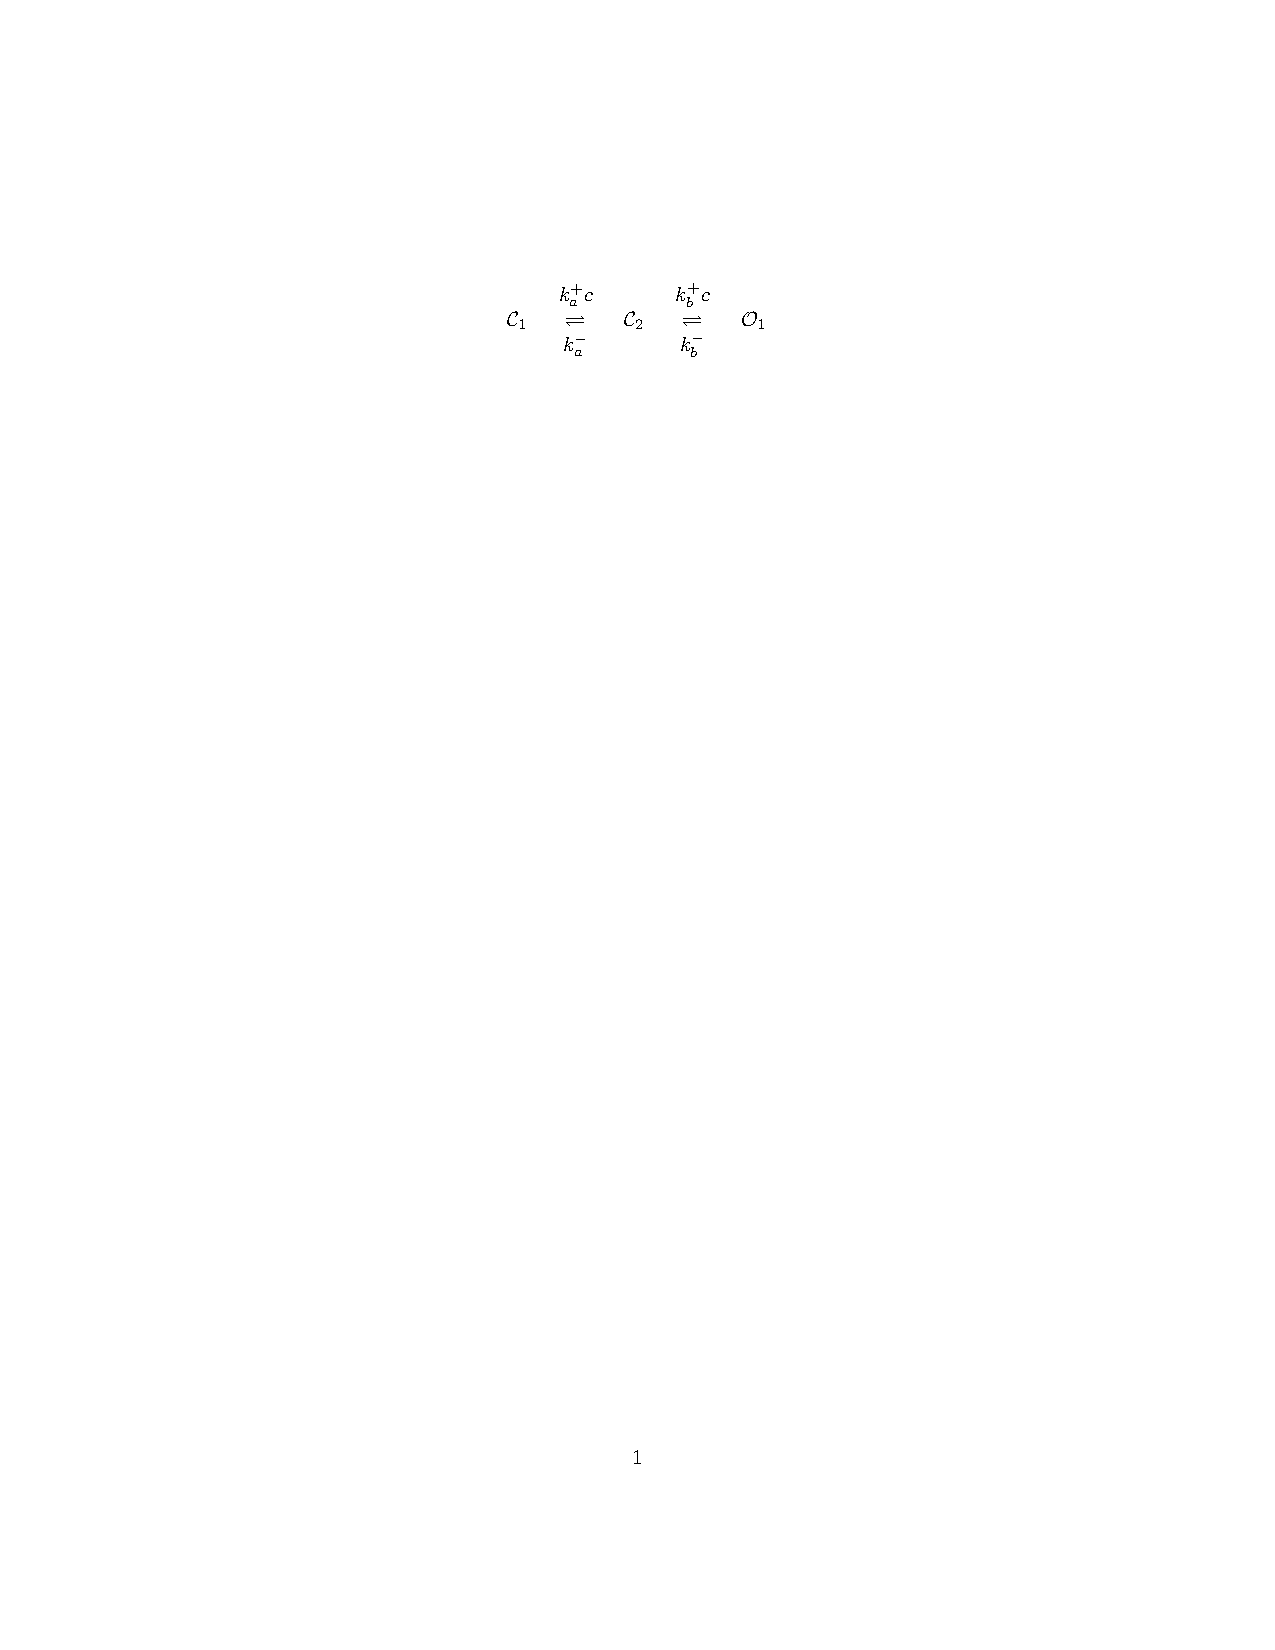
\includegraphics[height=1in]{pics/threestate}}

\end{picture}


%\caption{\small   \textbf{(a)} 3-state single channel model with \Ca-mediated activation that has two closed ($\mathcal{C}_1$, $\mathcal{C}_2$) and one open ($\mathcal{O}_1$) state. 
%Parameters in $\mu {\rm M}^{-1}\,{\rm ms}^{-1}$: $k_a^+$ = 1.5, $k_b^+$ = 150; in ${\rm ms}^{-1}$: $k_a^-$ = 50, $k_b^-$ = 1.5.  \textbf{(b)} 6-state single channel model with \Ca-mediated activation and inactivation. Parameters in $\mu {\rm M}^{-1}\,{\rm ms}^{-1}$: $k_a^+$ = 1.5, $k_b^+$ = $k_d^+$ = 0.015, $k_c^+$  =  $k_e^+$ =   300,  $k_f^+$ = 3.0; in ${\rm ms}^{-1}$: $k_a^-$ = 49.5, $k_b^-$ = $k_d^-$=  0.2475, $k_c^-$ =  $k_e^-$  = 6.0, $k_f^-$ = 0.03.
%}
%\vspace{-3.5in}
%\hspace{7in}
\vspace{2.5in}
\caption{Simultaneous measurement of \Ca\ changes in myoplasmic and jSR compartments during spontaneous sparks. $CASQ2^{WT}$, cells with overexpressed CSQ. $CASQ2^{DEL}$ , cells expressing mutant CSQ with reduced affinity for \Ca. $CASQ2^{R33Q}$, cells expressing mutant CSQ with reduced affinity for RyRs. Reproduced from [2].}
\label{fig:models}
\end{figure}
\end{center}
%\vspace{-9.85in}\hspace{-1.3in}\colorbox{white}{$\quad\quad\quad\quad\quad$ \small Control}
%\vspace{-8.1in}\colorbox{white}{\mbox{\hspace{8in}}}
%\PSFrame(5.5 ,3 , 5.8, 6, .5, APS_BLACK, APS_NONE, APS_CLEAR)




%%\medskip
%\begin{table}
%\footnotesize
%\centering
%\begin{tabular}{llccccccrrrrrrrr}
%\hline{\smallskip}
%${\mathrm{Solver}}$ && ${\mathrm{Max \ Res}}$ && ${\mathrm{Sum \ Res}}$ && ${\mathrm{CPU \ (s)}}$ &&  ${\mathrm{Wall \ (s)}}$ && ${\mathrm{Iters}}$ \\
%\noalign{\smallskip}
%\hline
%{\tt JOR} && {\tt9.49E-13} && {\tt5.16E-12}&& {\tt279}&& {\tt279} && {\tt1840} \\
%{\tt JOR\_AD} && {\tt9.44E-13} && {\tt5.13E-12}&& {\tt415}&& {\tt415} && {\tt1550 }\\
%{\tt ARNOLDI} && {\tt2.42E-13} && {\tt4.04E-11} && {\tt214} && {\tt215} && {\tt1440}\\
%{\tt BICGSTAB} && {\tt8.66E-13}  && {\tt4.89E-11}  && {\tt146} && {\tt148} && {\tt602}\\
%{\tt PRE\_ARNOLDI} && {\tt8.62E-15}  && {\tt1.82E-12 }&&{\tt 26}&&{\tt27} &&{\tt160} \\
%{\tt BSOR\_BICGSTAB} &&{\tt8.22E-15}&& {\tt5.29E-13} && {\tt19} && {\tt19}&& {\tt52} \\
%{\tt ML\_JOR\_F\_DYN} && {\tt5.87E-13} && {\tt1.68E-10} && {\tt15} && {\tt15} && {\tt46 }\\
%\hline
%\end{tabular}
%\caption{\small Benchmark calculations for 10 3-state channels.
%% computed using Linux PCs with dual core 3.8GHz EM64T Xeon processors and 8GB RAM solving \Eq{equ:kron}. 
%Description of solvers [1]: {\tt JOR}, Jacobi over-relaxation method; {\tt JOR\_AD}, method of Jacobi with aggregation/disaggregation; {\tt ARNOLDI}, method of Arnoldi; {\tt BICGSTAB}, biconjugate gradient stabilized method; {\tt PRE\_ARNOLDI}, method of Arnoldi with Neumann pre-conditioning; {\tt BSOR\_BICGSTAB}, biconjugate gradient stability method with block successive over-relaxation pre-conditioning; {\tt ML\_JOR\_F\_DYN}, multi-level method with {\tt JOR} smoother, F cycle, and dynamic ordering.}
% \label{THREESTATESUMMARY}
%\end{table}

%\medskip\hrule
\end{textblock}
%
%

%\begin{textblock}{5}(5.75, 0.8)
%%\hrule\medskip
%\Head{---Experimental results ---}
%\end{textblock}
%\begin{textblock}{2.0}(9.35,1.3)

%$\bold{Figure \  3:}$ Simultaneous measurement of \Ca\ changes during spontaneous sparks in myoplasmic and jSR domains. \\$CASQ2^{WT}$ mutants represent cells with overexpressed CSQ. $CASQ2^{DEL}$ mutants represent cells with CSQ that does not bind well to \Ca.\\ $CASQ2^{R33Q}$ mutants represent cells with CSQ that does not interact with RyRs.
%\end{textblock}

\begin{textblock}{6.0}(5.25,5.2)
\Head{--- Spark Simulation, Alignment, Averaging ---}
Simulated sparks were aligned and then averaged. The resulting emergent spark properties were compared to experimental observations of spark activity in control and CASQ2 mutant cells. Parameter studies were performed to test various aspects of the model against experimental evidence. Aspects of experiment replicated ({$\surd$}) or not replicated ({$\times$}) are shown to the right. Color in averaged simulated sparks indicates corresponding experimental results.
\end{textblock}

\begin{textblock}{6}(5.25,6.8)
%\Head{--- Simulated Sparks ---}
\vspace{0.3in}

\begin{center}
\begin{figure}
\begin{picture}(200,340)(200,340)
\put(-135,340){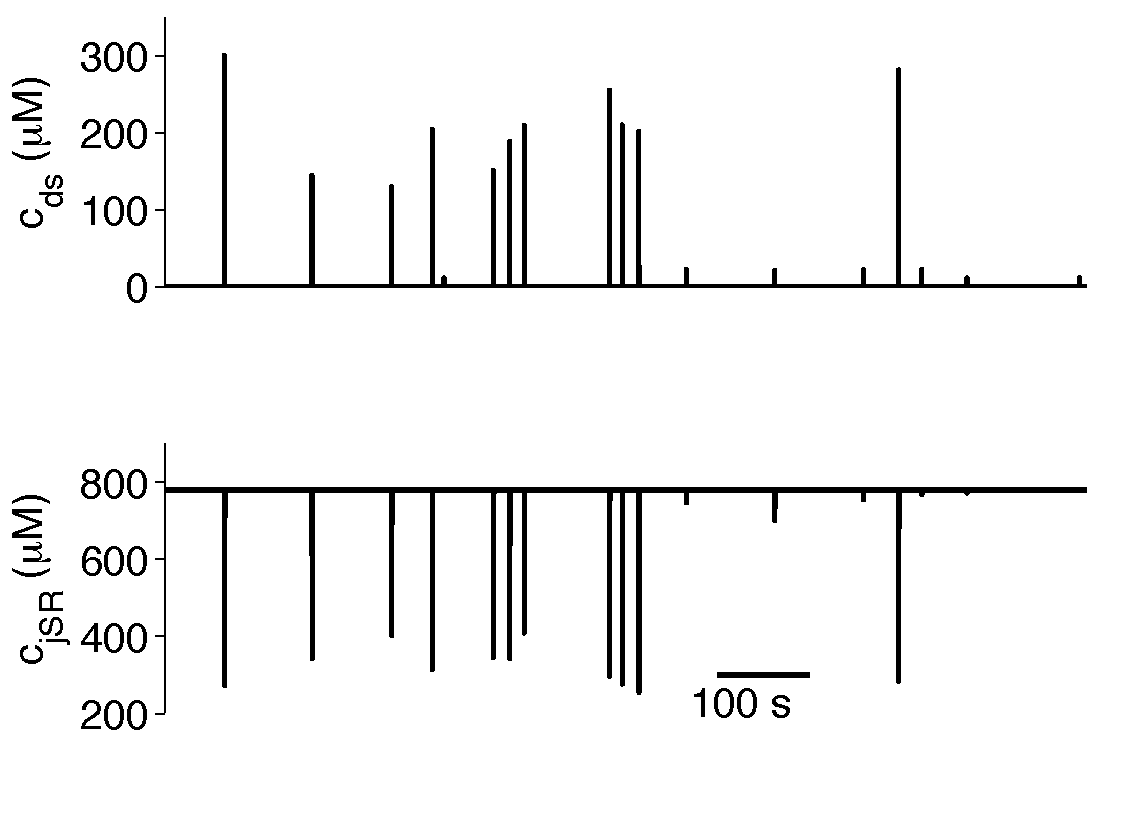
\includegraphics[height=4.5in]{pics/spark_trace_ca}}
\put(300,340){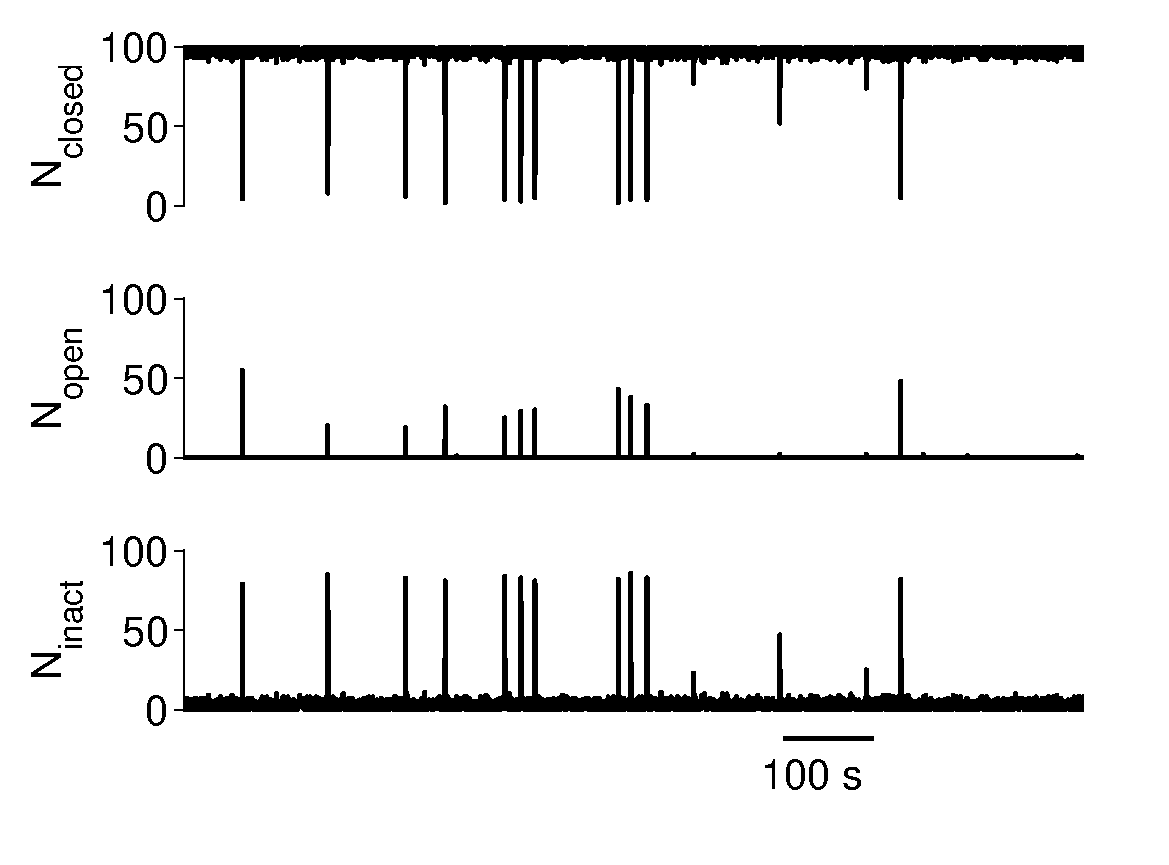
\includegraphics[height=4.5in]{pics/spark_trace_NEW_nstate}}
\put(-135,670){\scalebox{1.2}{(a)}}
\put(300,670){\scalebox{1.2}{(b)}}
%\put(-50,635){$\overbrace{\makebox[2.22in]{}}^{6-state}$}
%\put(60,423){$\underbrace{\makebox[3in]{}}_{3-state}$}
%\put(600,400){\scalebox{0.8}{\tt ML\_JOR\_F\_DYN}}
%\put(537,450){\thicklines \oval(20,50)}
%\put(586,412){\thicklines \vector(-2,1){40}}
%\put(600,500){\scalebox{0.8}{\tt Monte Carlo}}
%\put(730,585){\thicklines \oval(20,50)}
%\put(685,521){\thicklines \vector(1,1){40}}
\end{picture}

\vspace{-0.2in}
\caption{{\bf (a)} Representative times and amplitudes of spontaneous SR \Ca\ release and associated depletion signals exhibited by a \Ca\ release site model composed of 100 Lee-Keener RyRs.  {\bf (b)} Associated changes in channel state.}


%\caption{\small   {\bf (a):} Average cytosolic and SR [\Ca] for simulated and aligned sparks. The dashed, solid, and dotted lines correspond to $[CSQ]_T = 2.8$, $14$, and $70$ mM, respectively. 
%%Single-channel parameters as in \Fig{fig:models}.  Calculations performed using 2.66 GHz Dual-Core Intel Xeon processors and 2 GB RAM.  
%{\bf (b):} Average cytosolic and SR [\Ca] for simulated and aligned sparks. The dashed, solid, and dotted lines correspond to $[CSQ]_T = 2.8$, $14$, and $70$ mM, respectively.}
%Parameters as in ~\Fig{fig:sparks}.}
\label{fig:Spark_trace}
\end{figure}
\end{center}

\end{textblock}
%\begin{textblock}{5}(5.75,3.3)
%%\hrule\medskip
%\Head{--- Varying $[CSQ]_T$ ---}

%\begin{center}
%\begin{figure}
%\begin{picture}(200,340)(200,340)
%\put(-135,340){\includegraphics[height=4.5in]{pics/Vary_Y_ca}}
%\put(320,330){\includegraphics[height=4.5in]{pics/Vary_Y_nstate}}
%\put(-135,670){\scalebox{1.2}{(a)}}
%\put(320,665){\scalebox{1.2}{(b)}}
%%\put(-50,635){$\overbrace{\makebox[2.22in]{}}^{6-state}$}
%%\put(60,423){$\underbrace{\makebox[3in]{}}_{3-state}$}
%%\put(600,400){\scalebox{0.8}{\tt ML\_JOR\_F\_DYN}}
%%\put(537,450){\thicklines \oval(20,50)}
%%\put(586,412){\thicklines \vector(-2,1){40}}
%%\put(600,500){\scalebox{0.8}{\tt Monte Carlo}}
%%\put(730,585){\thicklines \oval(20,50)}
%%\put(685,521){\thicklines \vector(1,1){40}}
%\end{picture}

%\vspace{-0.2in}
%\caption{\small   {\bf (a):} Average cytosolic and SR [\Ca] for simulated and aligned sparks. The dashed, solid, and dotted lines correspond to $[CSQ]_T = 2.8$, $14$, and $70 mM$, respectively. 
%%Single-channel parameters as in \Fig{fig:models}.  Calculations performed using 2.66 GHz Dual-Core Intel Xeon processors and 2 GB RAM.  
%{\bf (b):} Average cytosolic and SR [\Ca] for simulated and aligned sparks. The dashed, solid, and dotted lines correspond to $[CSQ]_T = 2.8$, $14$, and $70$ mM, respectively.}
%%Parameters as in ~\Fig{fig:sparks}.}
%\label{fig:VARY_Y}
%\end{figure}
%\end{center}

%%\medskip\hrule
%\end{textblock}

\begin{textblock}{6}(5.25, 9.8)
%\hrule\medskip
\vspace{-0.4in}

%\Head{---Spark Alignment ---}
%\vspace{-0.2in}

\begin{center}
\begin{figure}
\begin{picture}(200,340)(200,340)
\put(-135,340){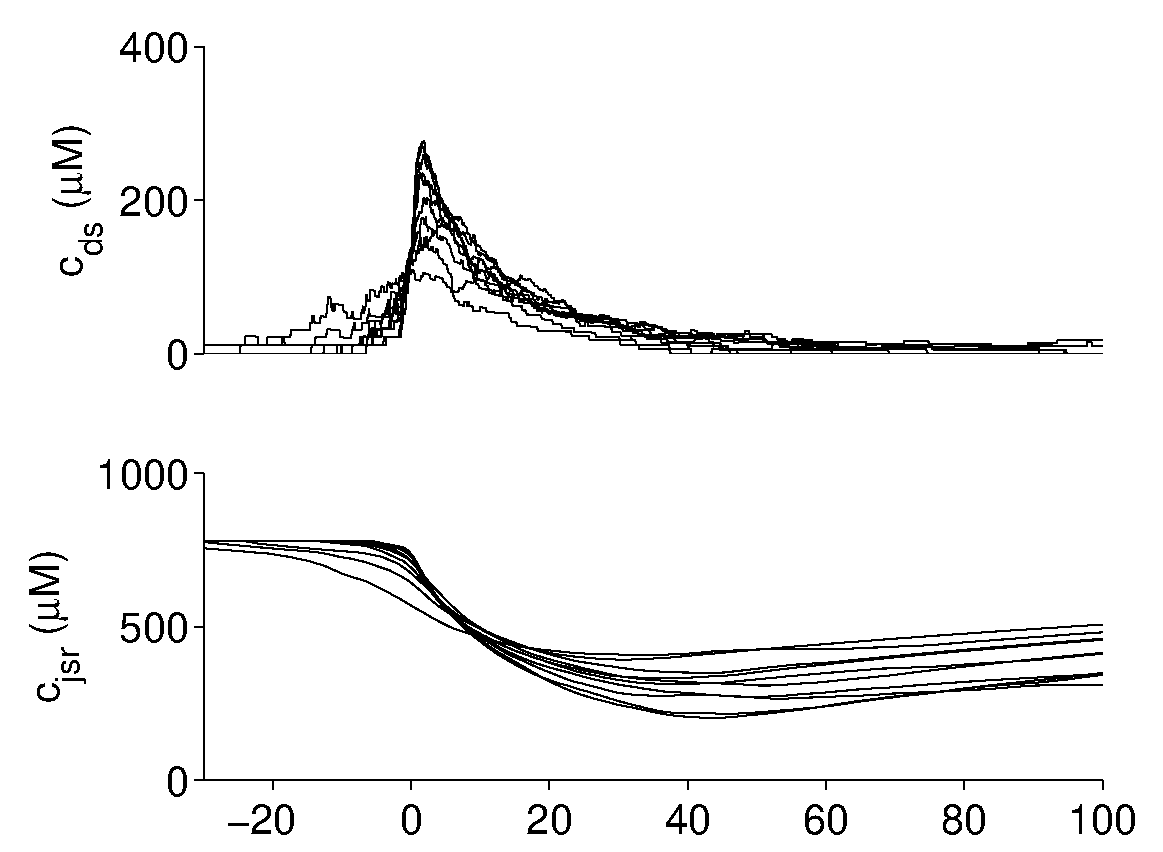
\includegraphics[height=4.5in]{pics/Aligned_few_color_ca}}
\put(300,330){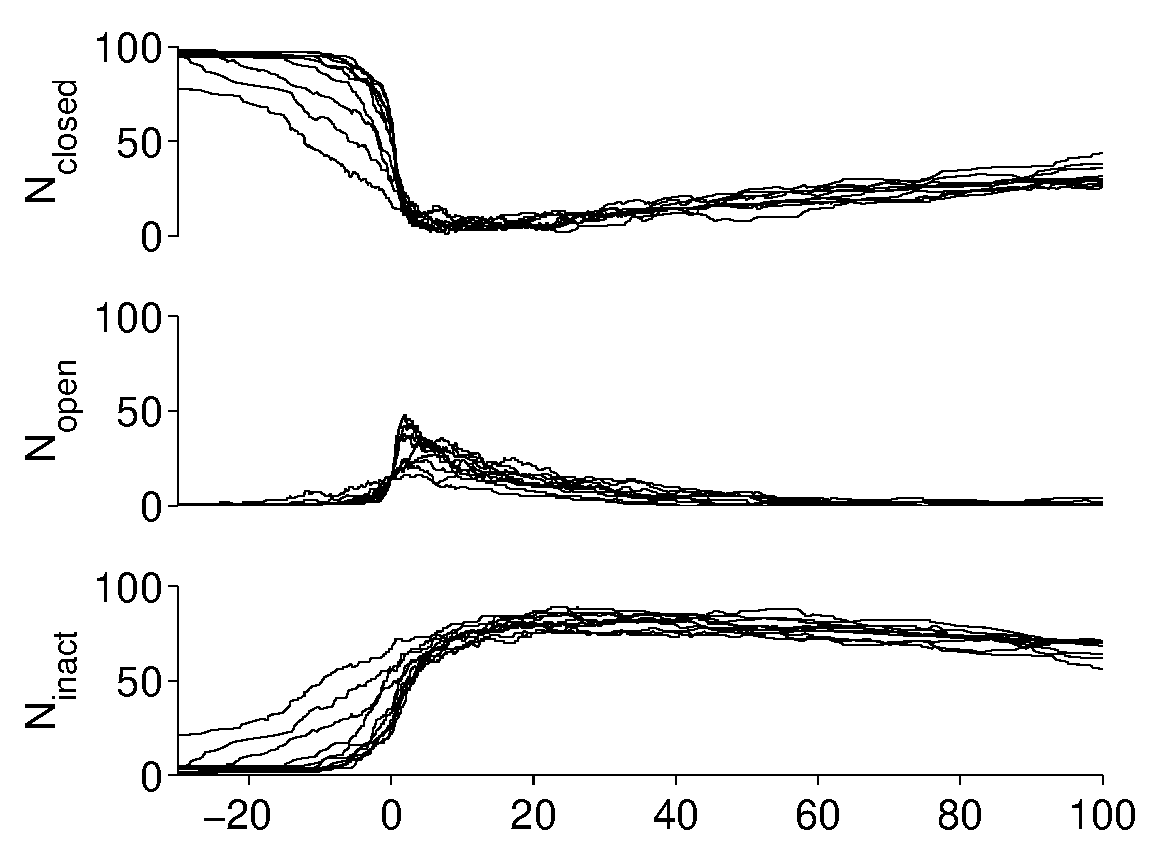
\includegraphics[height=4.5in]{pics/Aligned_few_poster_nstate}}


%\put(-135,340){\includegraphics[height=4.5in]{pics/aligned_sparks_ca}}
%\put(300,330){\includegraphics[height=4.5in]{pics/aligned_sparks_nstate}}
\put(-135,670){\scalebox{1.2}{(a)}}
\put(300,665){\scalebox{1.2}{(b)}}

\put(410,490){\scalebox{1.2}{$\searrow$}}
%\put(-50,635){$\overbrace{\makebox[2.22in]{}}^{6-state}$}
%\put(60,423){$\underbrace{\makebox[3in]{}}_{3-state}$}
%\put(600,400){\scalebox{0.8}{\tt ML\_JOR\_F\_DYN}}
%\put(537,450){\thicklines \oval(20,50)}
%\put(586,412){\thicklines \vector(-2,1){40}}
%\put(600,500){\scalebox{0.8}{\tt Monte Carlo}}
%\put(730,585){\thicklines \oval(20,50)}
%\put(685,521){\thicklines \vector(1,1){40}}
\end{picture}

\vspace{-0.2in}
\caption{Ten representative sparks aligned at the transition from 15 to 16 open channels (shown by arrow).  {\bf (a)} Diadic subspace and jSR [\Ca] as well as changes in {\bf (b)}  channel activity are shown.}


%\caption{\small   {\bf (a):} Average cytosolic and SR [\Ca] for simulated and aligned sparks. The dashed, solid, and dotted lines correspond to $K^{CSQ-Ca}_d = 127.6$, $638$, and $3190$ $\mu$ M, respectively. 
%%Single-channel parameters as in \Fig{fig:models}.  Calculations performed using 2.66 GHz Dual-Core Intel Xeon processors and 2 GB RAM.  
%{\bf (b):} Average cytosolic and SR [\Ca] for simulated and aligned sparks. The dashed, solid, and dotted lines correspond to $[CSQ]_T = 2.8$, $14$, and $70 mM$, respectively.}
%Parameters as in ~\Fig{fig:sparks}.}
\label{fig:aligned_sparks}
\end{figure}
\end{center}%\bigskip\hrule


%[[INSERT TEXT ABOUT PARAMETER STUDIES]] SHOULD INCLUDE APPROPRIATE PARAMETER STUDIES, HYPOTHESES, EXPECTATIONS, ETC. HOW THEY SHOULD RELATE TO EXPERIMENTS

\end{textblock}


%\begin{textblock}{5}(5.75, 9.3)
%%\hrule\medskip
%\Head{---Varying $K^{CSQ-RyR}_d$ ---}
%%\vspace{-0.2in}

%\begin{center}
%\begin{figure}
%\begin{picture}(200,340)(200,340)
%\put(-135,340){\includegraphics[height=4.5in]{pics/Vary_RYR_ca}}
%\put(320,330){\includegraphics[height=4.5in]{pics/Vary_RYR_nstate}}
%\put(-135,670){\scalebox{1.2}{(a)}}
%\put(320,665){\scalebox{1.2}{(b)}}
%%\put(-50,635){$\overbrace{\makebox[2.22in]{}}^{6-state}$}
%%\put(60,423){$\underbrace{\makebox[3in]{}}_{3-state}$}
%%\put(600,400){\scalebox{0.8}{\tt ML\_JOR\_F\_DYN}}
%%\put(537,450){\thicklines \oval(20,50)}
%%\put(586,412){\thicklines \vector(-2,1){40}}
%%\put(600,500){\scalebox{0.8}{\tt Monte Carlo}}
%%\put(730,585){\thicklines \oval(20,50)}
%%\put(685,521){\thicklines \vector(1,1){40}}
%\end{picture}

%\vspace{-0.2in}
%\caption{\small   {\bf (a):} Average cytosolic and SR [\Ca] for simulated and aligned sparks. The dashed, solid, and dotted lines correspond to $K^{CSQ-Ca}_d = 127.6$, $638$, and $3190$ $\mu$ M, respectively. 
%%Single-channel parameters as in \Fig{fig:models}.  Calculations performed using 2.66 GHz Dual-Core Intel Xeon processors and 2 GB RAM.  
%{\bf (b):} Average cytosolic and SR [\Ca] for simulated and aligned sparks. The dashed, solid, and dotted lines correspond to $[CSQ]_T = 2.8$, $14$, and $70 mM$, respectively.}
%%Parameters as in ~\Fig{fig:sparks}.}
%\label{fig:VARY_RYR}
%\end{figure}
%\end{center}%\bigskip\hrule

\begin{textblock}{5.0}(12.0, 0.8)
\Head{ --- $[CSQ]_T$ modulates spark activity ---}
\end{textblock}

\begin{textblock}{5.5}(11.75, 1.4)

%As $[CSQ]_T$ increases, spark amplitude increases, and jSR recovery time decreases.
%\begin{center}


\hspace{2in} {$\surd$} \labelitemi\ $[CSQ]_T \uparrow\ \Rightarrow$ spark amplitude $\uparrow$

\vspace{-0.1in} \hspace{2in} {$\surd$} \labelitemi\ $[CSQ]_T \uparrow\ \Rightarrow$ jSR recovery time $\uparrow$

\vspace{-0.1in} \hspace{2in}  {$\times$} \labelitemi\ $[CSQ]_T \uparrow\ \Rightarrow$ resting nSR [\Ca] and blink nadir $\uparrow$

\vspace{-0.1in} \hspace{2.35in} \labelitemi\ $[CSQ]_T \uparrow\ \Rightarrow$ channel activity is invariant


%\end{center}
\begin{center}
\begin{figure}
\begin{picture}(200,340)(200,340)
\put(-95,340){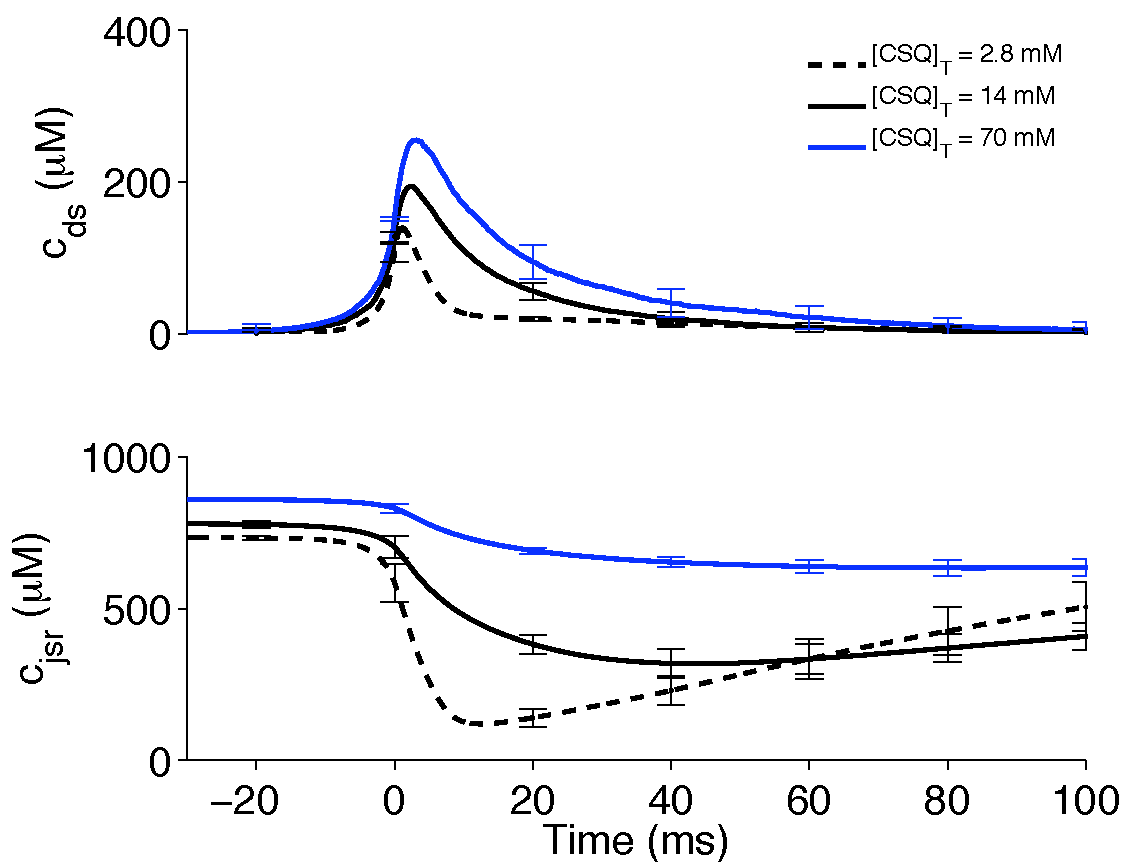
\includegraphics[height=4.25in]{pics/Vary_Y_ca_color_legend}}
\put(310,330){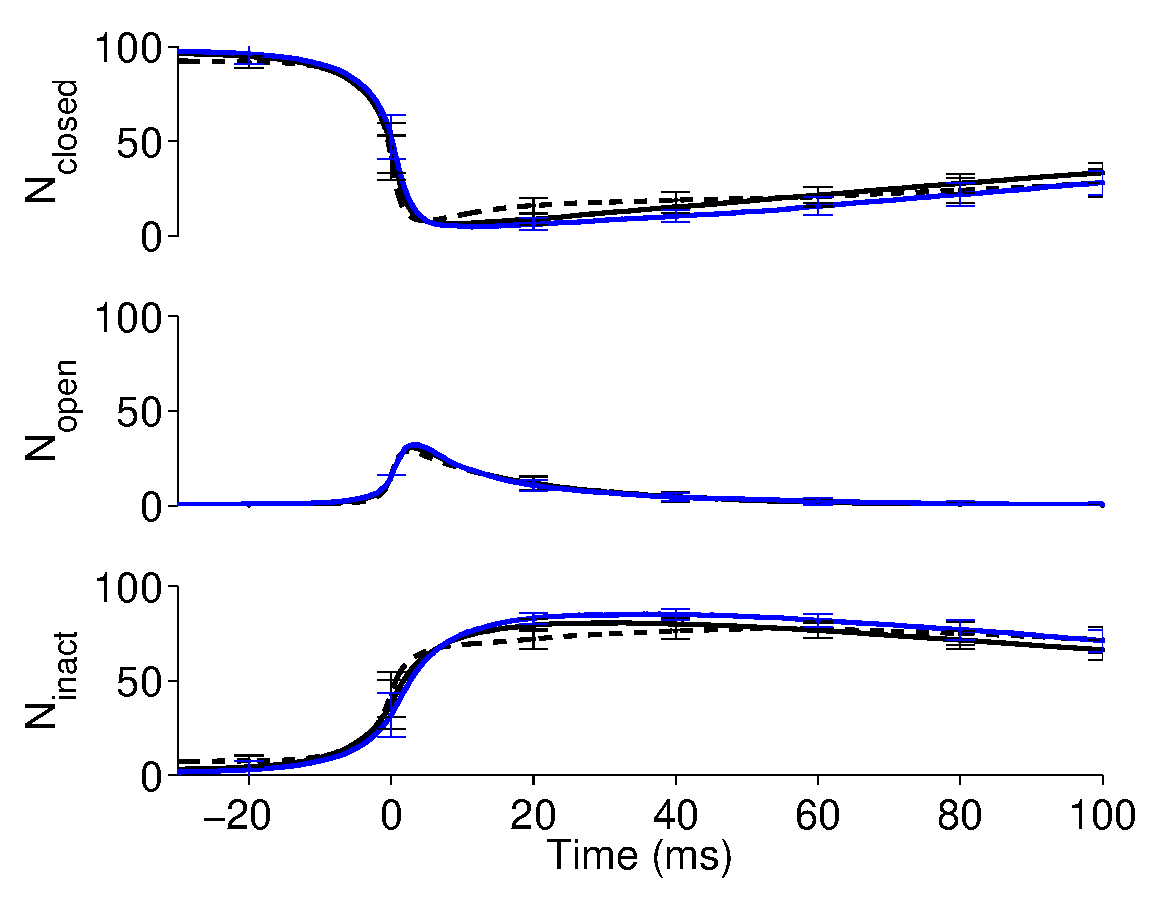
\includegraphics[height=4.25in]{pics/Vary_Y_poster_nstate}}
%\put(-95,670){\scalebox{1.2}{(a)}}
%\put(310,665){\scalebox{1.2}{(b)}}

%\put(-50,635){$\overbrace{\makebox[2.22in]{}}^{6-state}$}
%\put(60,423){$\underbrace{\makebox[3in]{}}_{3-state}$}
%\put(600,400){\scalebox{0.8}{\tt ML\_JOR\_F\_DYN}}
%\put(537,450){\thicklines \oval(20,50)}
%\put(586,412){\thicklines \vector(-2,1){40}}
%\put(600,500){\scalebox{0.8}{\tt Monte Carlo}}
%\put(730,585){\thicklines \oval(20,50)}
%\put(685,521){\thicklines \vector(1,1){40}}
\end{picture}

\vspace{-0.2in}
\caption{Average [\Ca] and channel activity for simulated sparks.}
%Parameters as in ~\Fig{fig:sparks}.}
\label{fig:VARY_Y}
\end{figure}
\end{center}

%\medskip\hrule
\end{textblock}


%\begin{textblock}{1}(12.20,4.85)
%\Head{---}
%\end{textblock}

%\begin{textblock}{1}(15.80,4.85)
%\Head{---}
%\end{textblock}

\begin{textblock}{5.5}(11.75, 4.4)
\Head{--- Reducing CSQ-\Ca\ affinity --- modulates spark activity}
\end{textblock}



\begin{textblock}{5.5}(11.75,5.2)


\hspace{2in} {$\surd$} \labelitemi\ $K_{CSQ-Ca}$ varies $\Rightarrow$ spark amplitude $\downarrow$

\vspace{-0.1in} \hspace{2in}  {$\surd$} \labelitemi\  $K_{CSQ-Ca}$ $\uparrow\ \Rightarrow$ jSR recovery time $\downarrow$

\vspace{-0.1in} \hspace{2in} {$\times$} \labelitemi\  $K_{CSQ-Ca}$ $\uparrow\ \Rightarrow$ resting nSR [\Ca] $\uparrow$


\vspace{-0.1in} \hspace{2.35in} \labelitemi\ $K_{CSQ-Ca}$ $\uparrow\ \Rightarrow N_{inact} \downarrow N_{C1} \uparrow$


\begin{center}
\begin{figure}
\begin{picture}(200,340)(200,340)
\put(-95,340){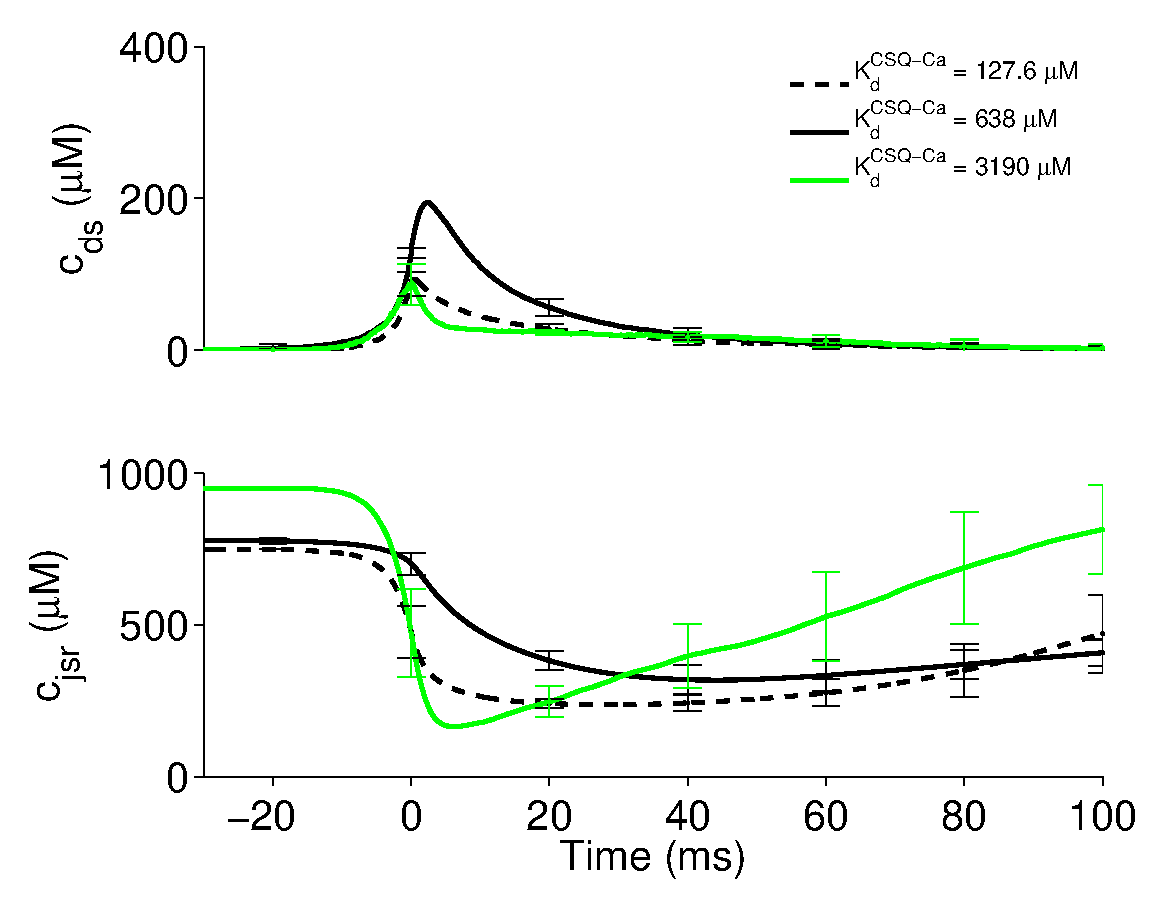
\includegraphics[height=4.25in]{pics/Vary_X_ca_color_legend}}
\put(310,330){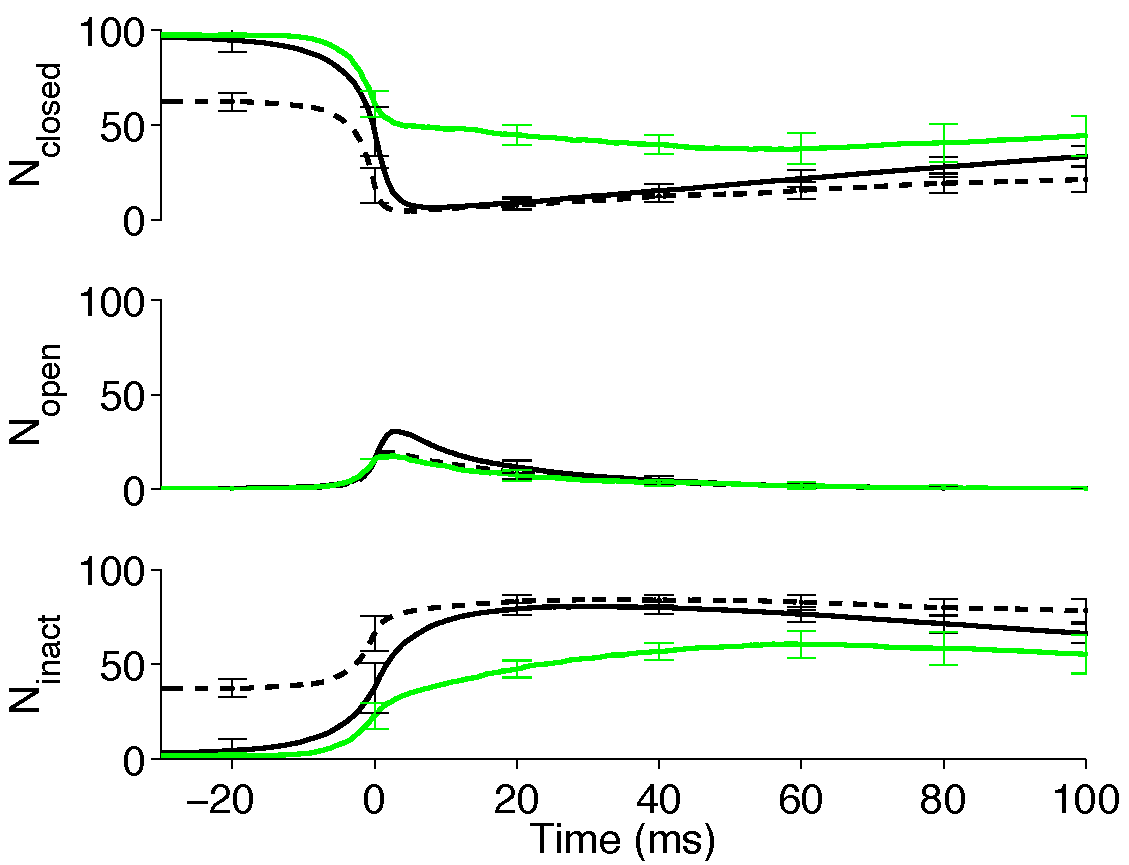
\includegraphics[height=4.25in]{pics/Vary_X_poster_nstate}}
%\put(-95,670){\scalebox{1.2}{(a)}}
%\put(310,665){\scalebox{1.2}{(b)}}

%\put(-50,635){$\overbrace{\makebox[2.22in]{}}^{6-state}$}
%\put(60,423){$\underbrace{\makebox[3in]{}}_{3-state}$}
%\put(600,400){\scalebox{0.8}{\tt ML\_JOR\_F\_DYN}}
%\put(537,450){\thicklines \oval(20,50)}
%\put(586,412){\thicklines \vector(-2,1){40}}
%\put(600,500){\scalebox{0.8}{\tt Monte Carlo}}
%\put(730,585){\thicklines \oval(20,50)}
%\put(685,521){\thicklines \vector(1,1){40}}
\end{picture}

\vspace{-0.2in}
\caption{Average [\Ca] and channel activity for simulated sparks.}
\label{fig:VARY_X}
\end{figure}
\end{center}

%\medskip\hrule
\end{textblock}

%\begin{textblock}{1}(12.20,8.65)
%\Head{---}
%\end{textblock}

%\begin{textblock}{1}(15.80,8.65)
%\Head{---}
%\end{textblock}

\begin{textblock}{5.5}(11.75, 8.4)
\Head{--- Reducing CSQ-RyR affinity --- modulates spark activity}
\end{textblock}


\begin{textblock}{5.5}(11.75,9.2)


\hspace{1.2in}  {$\surd$} \labelitemi\ $K_{CSQ-RyR} \uparrow$ $\Rightarrow$ amplitude \& average channel state invariant

\vspace{-0.1in} \hspace{1.2in} {$\surd$} \labelitemi\ $K_{CSQ-RyR}$ $\uparrow\ \Rightarrow$ resting nSR [\Ca] and blink nadir $\downarrow$


\begin{center}
\begin{figure}
\begin{picture}(200,340)(200,340)
\put(-95,340){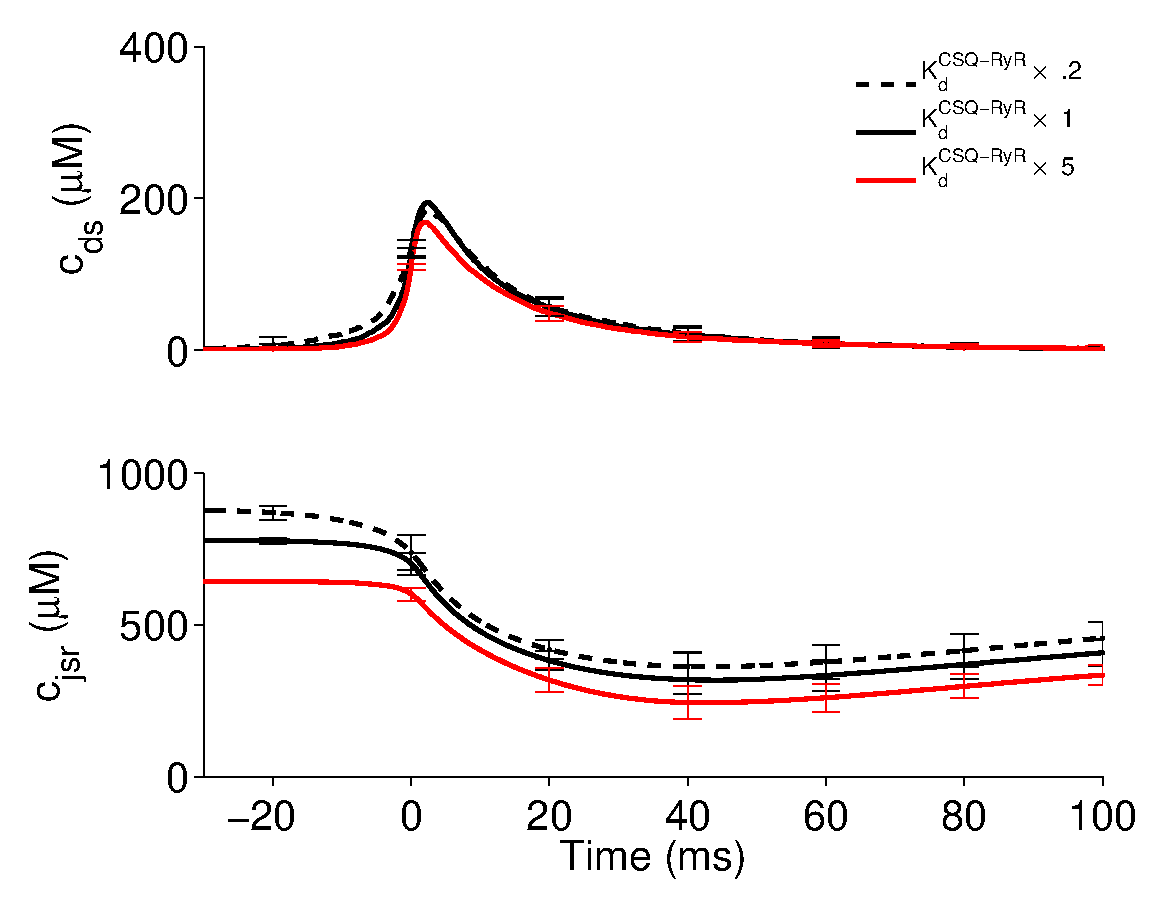
\includegraphics[height=4.25in]{pics/Vary_RYR_ca_color_legend}}
\put(310,330){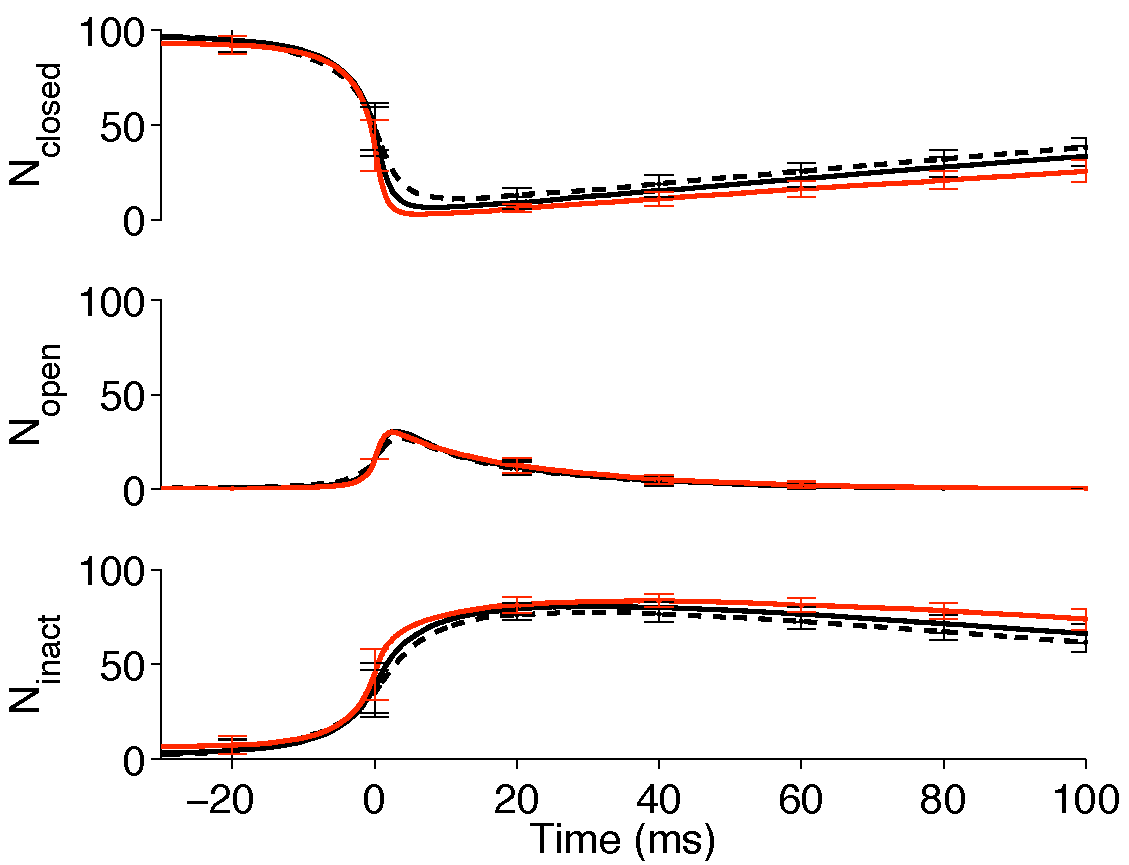
\includegraphics[height=4.25in]{pics/Vary_RYR_poster_nstate}}
%\put(-95,670){\scalebox{1.2}{(a)}}
%\put(310,665){\scalebox{1.2}{(b)}}

%\put(-50,635){$\overbrace{\makebox[2.22in]{}}^{6-state}$}
%\put(60,423){$\underbrace{\makebox[3in]{}}_{3-state}$}
%\put(600,400){\scalebox{0.8}{\tt ML\_JOR\_F\_DYN}}
%\put(537,450){\thicklines \oval(20,50)}
%\put(586,412){\thicklines \vector(-2,1){40}}
%\put(600,500){\scalebox{0.8}{\tt Monte Carlo}}
%\put(730,585){\thicklines \oval(20,50)}
%\put(685,521){\thicklines \vector(1,1){40}}
\end{picture}

\vspace{-0.2in}
\caption{Average [\Ca] and channel activity for simulated sparks.}
\label{fig:VARY_RYR}
\end{figure}
\end{center}

%\medskip\hrule
\end{textblock}
%\Head{--- Inactivation while varying $[CSQ]_T$---}

%
%\begin{center}
%\begin{figure}
%\begin{picture}(200,980)(200,340)

%\put(-90,1050){\includegraphics[height=4in]{pics/Vary_Y_slowkplus3_ca}}
%\put(320,1050){\includegraphics[height=4in]{pics/Vary_Y_slowkplus3_nstate}}
%\put(-90,740){\includegraphics[height=4in]{pics/Vary_Y_slowboth3_ca}}
%\put(320,740){\includegraphics[height=4in]{pics/Vary_Y_slowboth3_nstate}}
%\put(-90,430){\includegraphics[height=4in]{pics/Vary_Y_NoQ_ca}}
%\put(320,430){\includegraphics[height=4in]{pics/Vary_Y_NoQ_nstate}}

%

%\end{picture}
%\vspace{-1.2in}
%\caption{[[CAPTION]] [[CAPTION]] [[CAPTION]] [[CAPTION]] [[CAPTION]] [[CAPTION]] [[CAPTION]] [[CAPTION]] [[CAPTION]] [[CAPTION]] [[CAPTION]] [[CAPTION]] [[CAPTION]]}
%\label{fig:multi_fig}
%\end{figure}
%\end{center}

%
%\end{textblock}

%
%\begin{textblock}{5.5}(11.75,7.0)
%\Head{--- Inactivation while varying $K^{CSQ-Ca}_d$---}

%
%\begin{center}
%\begin{figure}
%\begin{picture}(200,980)(200,340)

%\put(-90,1050){\includegraphics[height=4in]{pics/Vary_X_slowkplus3_ca}}
%\put(320,1050){\includegraphics[height=4in]{pics/Vary_X_slowkplus3_nstate}}
%\put(-90,740){\includegraphics[height=4in]{pics/Vary_X_slowboth3_ca}}
%\put(320,740){\includegraphics[height=4in]{pics/Vary_X_slowboth3_nstate}}
%\put(-90,430){\includegraphics[height=4in]{pics/Vary_X_NoQ_ca}}
%\put(320,430){\includegraphics[height=4in]{pics/Vary_X_NoQ_nstate}}

%

%\end{picture}
%\vspace{-1.2in}
%\caption{[[CAPTION]] [[CAPTION]] [[CAPTION]] [[CAPTION]] [[CAPTION]] [[CAPTION]] [[CAPTION]] [[CAPTION]] [[CAPTION]] [[CAPTION]] [[CAPTION]] [[CAPTION]] [[CAPTION]]}
%\label{fig:multi_fig}
%\end{figure}
%\end{center}

%
%\end{textblock}



%
%\begin{textblock}{5.5}(17.75,0.3)
%\Head{--- Inactivation varying $K^{CSQ-RyR}_d$---}

%
%\begin{center}
%\begin{figure}
%\begin{picture}(200,980)(200,340)

%\put(-90,1050){\includegraphics[height=4in]{pics/Vary_RYR_slowkplus3_ca}}
%\put(320,1050){\includegraphics[height=4in]{pics/Vary_RYR_slowkplus3_nstate}}
%\put(-90,740){\includegraphics[height=4in]{pics/Vary_RYR_slowboth3_ca}}
%\put(320,740){\includegraphics[height=4in]{pics/Vary_RYR_slowboth3_nstate}}
%\put(-90,430){\includegraphics[height=4in]{pics/Vary_RYR_NoQ_ca}}
%\put(320,430){\includegraphics[height=4in]{pics/Vary_RYR_NoQ_nstate}}

%

%\end{picture}
%\vspace{-1.2in}
%\caption{[[CAPTION]] [[CAPTION]] [[CAPTION]] [[CAPTION]] [[CAPTION]] [[CAPTION]] [[CAPTION]] [[CAPTION]] [[CAPTION]] [[CAPTION]] [[CAPTION]] [[CAPTION]] [[CAPTION]]}
%\label{fig:multi_fig}
%\end{figure}
%\end{center}

%
%\end{textblock}


%\begin{textblock}{1}(17.90,0.55)
%\Head{---}
%\end{textblock}

%\begin{textblock}{1}(22.10,0.55)
%\Head{---}
%\end{textblock}

\begin{textblock}{4.5}(18.25, 0.3)
\Head{--- Effects of CSQ buffering on --- spark activity}
\end{textblock}


\begin{textblock}{5.5}(17.75,1.1)

%\Head{--- Varying $K_{CSQ-RyR}$ and $[CSQ]_T$ ---}

\hspace{1.5in} \labelitemi\ $K_{CSQ-RyR}\  \&\ [CSQ]_T \uparrow$ $\Rightarrow$ amplitude $\uparrow$

\vspace{-0.1in} \hspace{1.5in} \labelitemi\ $K_{CSQ-RyR}\  \&\ [CSQ]_T  \uparrow\ \Rightarrow$ $N_{inact} \uparrow \ N_{C1} \downarrow$

\begin{center}
\begin{figure}
\begin{picture}(200,340)(200,340)
\put(-95,340){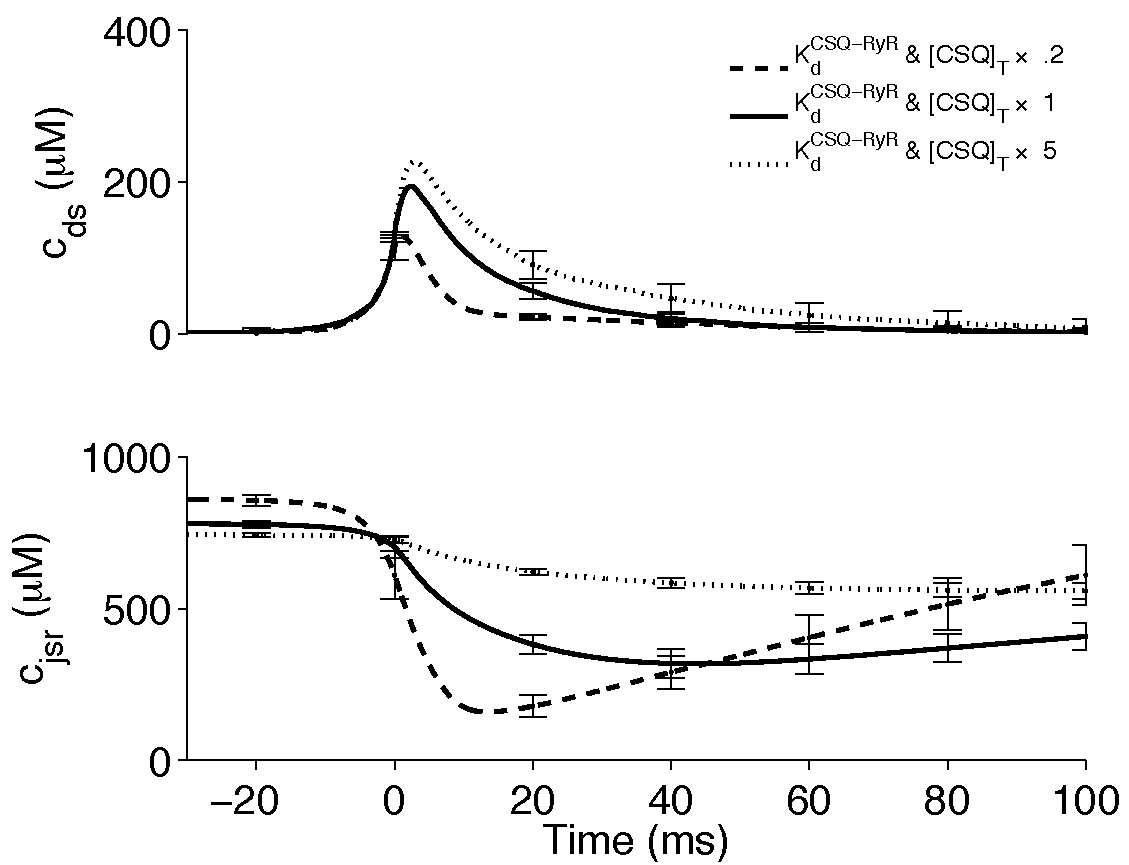
\includegraphics[height=4.25in]{pics/Vary_Y_RYR_ca_legend}}
\put(310,330){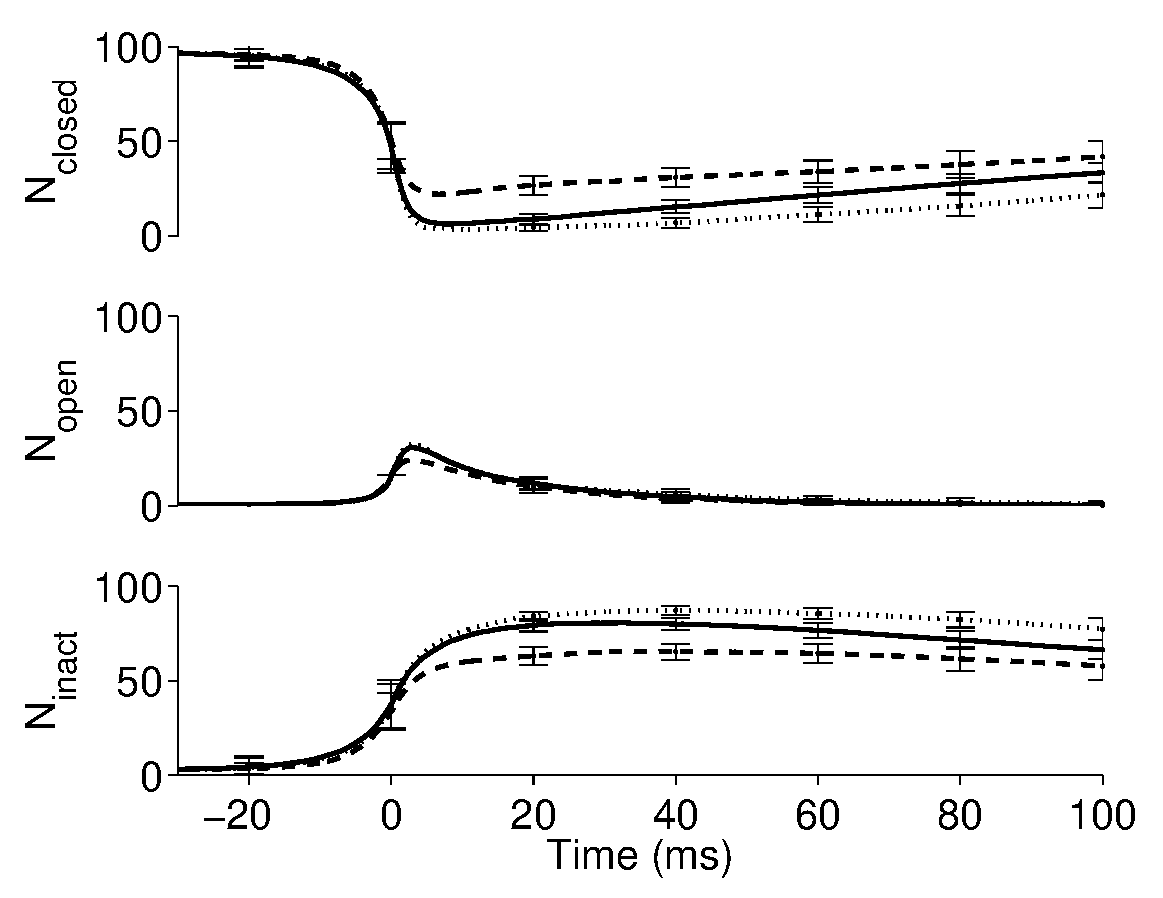
\includegraphics[height=4.25in]{pics/Vary_Y_RYR_poster_nstate}}
%\put(-95,670){\scalebox{1.2}{(a)}}
%\put(310,665){\scalebox{1.2}{(b)}}

%\put(-50,635){$\overbrace{\makebox[2.22in]{}}^{6-state}$}
%\put(60,423){$\underbrace{\makebox[3in]{}}_{3-state}$}
%\put(600,400){\scalebox{0.8}{\tt ML\_JOR\_F\_DYN}}
%\put(537,450){\thicklines \oval(20,50)}
%\put(586,412){\thicklines \vector(-2,1){40}}
%\put(600,500){\scalebox{0.8}{\tt Monte Carlo}}
%\put(730,585){\thicklines \oval(20,50)}
%\put(685,521){\thicklines \vector(1,1){40}}
\end{picture}

\vspace{-0.2in}
\caption{Average [\Ca] and channel activity for simulated sparks. Both $K_{CSQ-RyR}$ and $[CSQ]_T$ are modified so that the proportion of CSQ bound to the channel would be invariant over different parameters. This allows a focus on differences in spark statistics based purely on the buffering properties of CSQ.}
%Parameters as in ~\Fig{fig:sparks}.}
\label{fig:VARY_Y_RYR}
\end{figure}
\end{center}

%\medskip\hrule
\end{textblock}


\begin{textblock}{5.5}(17.75,4.3)
\Head{--- RyR inactivation studies ---}

\labelitemi\ The Lee-Keener RyR model includes CSQ-mediated facilitation of cytosolic \Ca\ inactivation as well as CSQ-mediated suppression of cytosolic \Ca\ activation.  The direct inactivation of the RyR by CSQ is a possible mechanism that is not included in the Lee-Keener model.  Further studies were performed to ascertain how these mechanisms may determine CSQ's role in regulating spontaneous \Ca\ release.

\labelitemi\ Direct inactivation of channels by CSQ results in fewer open channels and an associated rise in the number of closed channels. This results in lower spark amplitudes with few changes in associated blinks, as well as the inability of sparks to initiate (not shown).

\labelitemi\ Down-regulation of inactivation via cytosolic \Ca\ resulted in the inability of CSQ to regulate the channel effectively. Sparks were often terminated as a result of luminal depletion (not shown).


\end{textblock}


\begin{textblock}{5.5}(17.75,7.1)
\Head{--- Conclusions ---}

\labelitemi\ The effect of CSQ on modulating RyR activity was studied in a \Ca\ release site model composed of 100 Lee-Keener RyRs coupled with a bidomain model of spontaneous \Ca\ release.

\labelitemi\ Many aspects of experimental evidence of CSQ mutations are replicated by the model. However, certain key features, such as blink nadir and resting nSR [\Ca] in specific mutants are not observed. Thus, a constant blink nadir regardless of CSQ buffering strength might not be associated with a luminal \Ca-dependent spark termination mechanism.

\labelitemi\ The buffering properties of CSQ have an effect on the change in resting nSR [\Ca], by modulating the spark amplitude. However, the binding of CSQ to the RyR causes spark frequency to fall, which overshadows the effects of spark amplitude on resting nSR [\Ca].

%\labelitemi varying $CSQ_T$ - the increase in spark amplitude has more to do with CSQ buffering aspects, than the ability to close channels, as evidenced by the lack of change in the number of channels in each state. However, slowing down the role of Ca inactivation affects the number of channels in the open state, which gives rise to a further increase in spark amplitude. Having CSQ directly inactivate the channel rather than facilitate inactivation causes a decline in the number of open channels overall, but not between differing $[CSQ]_T$.

%varying $K^{CSQ-Ca}_d$ - 
%Kd high - luminal depletion plays a role... but also half as many channels activated
%Kd normal - high amount of activation by Ca
%Kd low - significantly more inactivated channels at rest
%slowing Ca inact - less channels open for varied Kd (slowing both ways causes very little channels to activate... but also massively depletes the lumen.
%noQ - same number of channels open, but different amplitudes - (buffering properties, although increased inactivated channels...)

%varying $K^{CSQ-RyR}_d$ - 
%no changes in channel activity... no changes in spark amplitude. resting nSR [Ca] changes as expected. high Kd => less binding => lower resting nSR
%slowing Ca inact - depletion is much much slower, slightly different spark amplitudes for slowkplus
%slowing both  - no changes in channel activity or spark amplitude (changes in nSR)
%noQ - high Kd gives slightly more open and inactivated channels, and a lower nSR





\end{textblock}

%\begin{textblock}{5.5}(17.75,12.0)

%Figure 9: [[CAPTION]] [[CAPTION]] [[CAPTION]] [[CAPTION]] [[CAPTION]] [[CAPTION]] [[CAPTION]] [[CAPTION]] [[CAPTION]] [[CAPTION]] [[CAPTION]] [[CAPTION]] [[CAPTION]]
%\end{textblock}
%
%\begin{textblock}{5.5}(17.75,0.45)
%%\hrule\medskip
%\Head{--- Effects of CSQ inactivation  ---}
%% NOT COMPLETELY RIGHT!!!!!
%\begin{center}
%\begin{figure}
%\begin{picture}(200,680)(200,340)
%\put(-135,670){\includegraphics[height=4in]{pics/Vary_X_NoQ_ca}}
%\put(350,670){\includegraphics[height=4in]{pics/Vary_X_NoQ_nstate}}
%\put(-135,340){\includegraphics[height=4in]{pics/Vary_Y_NoQ_ca}}
%\put(350,340){\includegraphics[height=4in]{pics/Vary_X_NoQ_nstate}}
%\put(-135,340){\includegraphics[height=4in]{pics/Vary_RYR_NoQ_ca}}
%\put(350,340){\includegraphics[height=4in]{pics/Vary_RYR_NoQ_nstate}}
%\put(-165,670){\scalebox{1.2}{(a)}}
%\put(320,665){\scalebox{1.2}{(b)}}
%%\put(-50,635){$\overbrace{\makebox[2.22in]{}}^{6-state}$}
%%\put(60,423){$\underbrace{\makebox[3in]{}}_{3-state}$}
%%\put(600,400){\scalebox{0.8}{\tt ML\_JOR\_F\_DYN}}
%%\put(537,450){\thicklines \oval(20,50)}
%%\put(586,412){\thicklines \vector(-2,1){40}}
%%\put(600,500){\scalebox{0.8}{\tt Monte Carlo}}
%%\put(730,585){\thicklines \oval(20,50)}
%%\put(685,521){\thicklines \vector(1,1){40}}
%\end{picture}

%\vspace{-0.2in}
%\caption{\small   {\bf (a):} Average cytosolic and SR [\Ca] for simulated and aligned sparks. The dashed, solid, and dotted lines correspond to $K^{CSQ-Ca}_d = 127.6$, $638$, and $3190$ $\mu$ M, respectively. 
%%Single-channel parameters as in \Fig{fig:models}.  Calculations performed using 2.66 GHz Dual-Core Intel Xeon processors and 2 GB RAM.  
%{\bf (b):} Average cytosolic and SR [\Ca] for simulated and aligned sparks. The dashed, solid, and dotted lines correspond to $[CSQ]_T = 2.8$, $14$, and $70 mM$, respectively.}
%%Parameters as in ~\Fig{fig:sparks}.}
%\label{fig:VARY_RYR}
%\end{figure}
%\end{center}%\bigskip\hrule
%%\medskip\hrule
%\end{textblock}

%\begin{textblock}{7.5}(15.75,3.2)
%%\hrule\medskip
%\Head{--- Approximate Methods: Scalability and Error ---}

%\begin{center}
%\begin{figure}
%\includegraphics[height=6in]{pics/figure6a_6b}
%\vspace{-0.3in}
%\caption{\small   \textbf{(a)} %Statistics for a release site composed of 12 3-state channels.  Left: Local [\Ca] near $3\times 3$ \Um\ ER membrane modeled as in \Fig{fig:sparks}.  Middle: Localized \Ca\ elevations reminiscent of \Ca\ puffs/sparks.  Right: 
%Probability distribution of the number of open channels calculated exactly using {\tt ML\_JOR\_F\_DYN} ({\it black bars}) and approximately using {\tt APP\_POWER} with  $\CO$ partitioning ({\it white bars}).  \textbf{(b)} Statistics as in (a) for 8 6-state channels with {\it black bars} denoting {\tt ML\_JOR\_F\_DYN} and {\it white and grey bars} denoting {\tt APP\_POWER} with $\CO$ and $\CRO$ partitioning, respectively.}
%\label{fig:appsparks}
%\end{figure}
%\end{center}

%\begin{center}
%\begin{figure}
%\begin{picture}(400,430)(400,430)
%\put(150,420){\includegraphics[height=6in]{pics/figure7a_7b}}
%\put(420,525){\scalebox{0.8}{{\it Filled}: \ {\tt APP\_POWER}}}
%\put(420,505){\scalebox{0.8}{{\it Open}: \ Exact Methods}}
%\put(870,525){\scalebox{0.8}{{\it Filled}: \ {\tt APP\_POWER}}}
%\put(870,505){\scalebox{0.8}{{\it Open}: \ Monte Carlo}}
%\end{picture}

%\vspace{-0.2in}
%\caption{\small   \textbf{(a)} {\it Filled} and {\it open} symbols show the wall clock time for the 6-state model (\Fig{fig:sparks}(d)).
%%using approximate and exact methods, respectively. 
%Approximate results are shown for two levels of partitioning ($\CO$, {\it squares} and $\CRO$, {\it circles}) with the {\tt APP\_POWER} method. Exact solutions are calculated using the {\tt POWER} method ({\it squares}) and {\tt ML\_JOR\_F\_DYN} method ({\it circles}).    \textbf{(b)} Results as in (a) with {\it open} symbols benchmarking Monte Carlo estimates of the distribution of $N_{\mathcal{O}}$ ({\it circles}) and the distribution of probability across the $M$ states of an arbitrary individual channel ({\it squares}). The {\it dashed line} shows the projected performance of an  approximate multi-level solver that uses {\tt ML\_JOR\_F\_DYN} rather than  {\tt POWER} as its iterative engine.}
%\label{fig:appsparks}
%\end{figure}
%\end{center}

%%\medskip\hrule
%\end{textblock}

\begin{textblock}{5.5}(17.75,9.7)
%\hrule\medskip
\Head{--- References ---}
\vspace{-0.3in}
\begin{description}

\item{[1]}  Y.-S. Lee and J. P. Keener. A calcium-induced calcium release mechanism mediated by calsequestrin \textit{J Theor Biol}, 253:668 - 679, Jan 2008.

\item{[2]} \ D. Terentyev, et al. Modulation of sr ca release by luminal ca and calsequestrin in cardiac myocytes: Effects of casq2 mutations linked to sudden cardiac death \textit{Biophys J}, 95:2037 - 2048, Jan 2008. 


%\item{[1]} \ W. Stewart, \textit{Introduction to the numerical solution of Markov chains}, Princeton: Princeton University Press (1994).

%\item{[4]} H. DeRemigio, P. Kemper, M. D. LaMar, and G. D. Smith, \textit{Markov chain models of coupled intracellular calcium channels: Kronecker structured representations and benchmark stationary distribution calculations}, Pacific Symposium on Biocomputing (2008), pp. 354--365.
\end{description} 

\begin{wrapfigure}{r}{1.5in}
\begin{center}

%\begin{picture}(280,340)(280,680)
%\put(180,660)
{\includegraphics[height=1.5in]{pics/NSF_correct_logo}}
%\end{picture}
%\caption{\small {CAPTION}}
\label{fig:CSQ}
\end{center}
\end{wrapfigure}
This material is based upon work supported by the National Science Foundation under Grant No. 0443843.
%\medskip\hrule
\end{textblock}

\begin{textblock}{1}(19.00,11.5)
\begin{figure}
\includegraphics[height=2in]{pics/CBLlogo2}
\end{figure}
\end{textblock}

%\begin{textblock}{1}(19.00,11.5)
%\begin{center}
%\begin{figure}
%\begin{picture}(280,340)(280,680)
%\put(180,660){\includegraphics[height=2in]{pics/CBLlogo}}
%\end{picture}
%%\caption{\small {Schematic representation of model components and fluxes. The model includes domain [\Ca] as well as bulk [\Ca]}}
%\label{fig:domains}
%\end{figure}
%\end{center}
%\end{textblock}

%\begin{textblock}{23}(0, 12.25)
%%\hrule\medskip
%\begin{center}
%\color{DarkBlue}
%The authors thank Buchholz and Dayar for sharing their implementation of Nsolve. This material is based upon work supported by the National Science Foundation under Grants 0133132 and 0443843.
%\end{center}
%%\medskip\hrule
%\end{textblock}

%\begin{textblock}{23}(3.3,12.1)
%\begin{figure}
%\includegraphics[height=1.5in]{pics/NSFlogo}
%\end{figure}
%\end{textblock}

%\begin{textblock}{1}(19.1,12.1)
%\begin{figure}
%\includegraphics[height=1.5in]{pics/NSFlogo}
%\end{figure}
%\end{textblock}

\end{document}
